\documentclass[hideothersubsections, usenames,dvipsnames,11pt]{beamer}
%%%%%%%%%%%%%%%%%%%%%%%%%%%%%%%%%%%%%%%%%%%%%%%%%%%%%%%%%%%%%%%%%%%%%%%%%%%%%%%%%%%%%%%%%%%%%%%%%%%%%%%%%%%%%%%%%%%%%%%%%%%%%%%%%%%%%%%%%%%%%%%%%%%%%%%%%%%%%%%%%%%%%%%%%%%%%%%%%%%%%%%%%%%%%%%%%%%%%%%%%%%%%%%%%%%%%%%%%%%%%%%%%%%%%%%%%%%%%%%%%%%%%%%%%%%%
\usepackage{algorithm}
\usepackage{algorithmic}
\usepackage{amsmath}
\usepackage{amssymb}
\usepackage{curves}
\usepackage{epic}
\usepackage{epsfig}
\usepackage{fix-cm}
\usepackage{graphicx}
\usepackage{hyperref}
\usepackage{mathpazo}
\usepackage{multimedia}
\usepackage{multicol}
\usepackage{natbib}
\usepackage{setspace}



\setcounter{MaxMatrixCols}{10}
%TCIDATA{OutputFilter=LATEX.DLL}
%TCIDATA{Version=5.00.0.2606}
%TCIDATA{Codepage=932}
%TCIDATA{<META NAME="SaveForMode" CONTENT="1">}
%TCIDATA{BibliographyScheme=Manual}
%TCIDATA{Created=Friday, November 03, 2006 10:56:24}
%TCIDATA{LastRevised=Thursday, February 19, 2015 11:02:18}
%TCIDATA{<META NAME="GraphicsSave" CONTENT="32">}
%TCIDATA{<META NAME="DocumentShell" CONTENT="Other Documents\SW\Slides - Beamer">}
%TCIDATA{Language=American English}
%TCIDATA{CSTFile=beamer.cst}

\newenvironment{stepenumerate}{\begin{enumerate}[<+->]}{\end{enumerate}}
\newenvironment{stepitemize}{\begin{itemize}[<+->]}{\end{itemize} }
\newenvironment{stepenumeratewithalert}{\begin{enumerate}[<+-| alert@+>]}{\end{enumerate}}
\newenvironment{stepitemizewithalert}{\begin{itemize}[<+-| alert@+>]}{\end{itemize} }
\newenvironment{itemize_2pt}{\itemize\addtolength{\itemsep}{2pt}}{\enditemize}
\newenvironment{enumerate_2pt}{\enumerate\addtolength{\itemsep}{2pt}}{\endenumerate}


% Color scheme
\definecolor{cerulean}{rgb}{0.16, 0.32, 0.75}
\definecolor{bdf}{rgb}{0.19, 0.55, 0.91}
\definecolor{offwhite}{RGB}{255,253,243}
\definecolor{red}{RGB}{213,94,0}
\definecolor{camel}{rgb}{0.76, 0.6, 0.42}
%#09BADB #DB1A71

\usetheme[right]{Berkeley}
\setbeamercolor{background canvas}{bg=offwhite}
\setbeamercolor{palette primary}{bg=cerulean,fg=white}
\setbeamercolor{palette secondary}{bg=bdf,fg=white}
\setbeamercolor{frametitle}{fg=offwhite}
%\setbeamercolor{sidebar}{bg=cerulean}
%\newenvironment{transitionframe}{\setbeamercolor{background canvas}{bg=bdf}\begin{frame}}{\end{frame}}
%\setbeamercolor{title}{fg=black}
%\setbeamercolor{itemize item}{fg=blue}
%\setbeamercolor{itemize subitem}{fg=blue}
%\setbeamercolor{enumerate item}{fg=blue}
%\setbeamercolor{enumerate subitem}{fg=blue}
%\setbeamercolor{title}{bg=red!25!blue,fg=white}
%\setbeamercolor{fo} {bg=red!25!blue,fg=white}
%\setbeamercolor{sidebar}{bg=red!25!blue,fg=white}
%\setbeamercolor{author in sidebar}{fg=black!20!white}
%\setbeamercolor{title in sidebar}{fg=white}
%\setbeamercolor{normal text}{bg=white}
%\setbeamercolor{frametitle}{fg=white}
%\setbeamercolor{section in sidebar}{bg=black,fg=white}
%\setbeamercolor{subsection in sidebar}{bg=black,fg=white}
%\setbeamercolor{block title}{bg=red!25!blue,fg=white}
%\setbeamercolor{block body}{bg=blue!20!white,fg=black}
%\setbeamerfont{subsection in sidebar}{size=\tiny}
%\setbeamerfont{title in sidebar}{size=\scriptsize}
%\setbeamerfont{author in sidebar}{size=\tiny}
%\setbeamercovered{transparent}
\setbeamercolor{section in sidebar}{bg=bdf,fg=offwhite}
\setbeamercolor{subsection in sidebar}{bg=bdf,fg=offwhite}
\setbeamercolor{button}{bg=bdf,fg=offwhite}


% Create subsection transitions without subsection numbering
\def\subsectionname{\translate{Subsection}}
\def\insertsubsectionnumber{\arabic{subsection}}
\setbeamertemplate{subsection page}
{
  %\begin{centering}
    %{\usebeamerfont{subsection name}\usebeamercolor[fg]{subsection name}\subsectionname~\insertsubsectionnumber}
    %\vskip1em\par
    \begin{beamercolorbox}[sep=14pt,center]{part title}
    	%\setbeamercolor{box1}{fg=yellow, bg=yellow}
    	\setbeamerfont{subsection title}{size=\fontsize{14}{20}\selectfont}
    	\usebeamerfont{subsection title}\insertsubsection\par
    \end{beamercolorbox}
  %\end{centering}
}
\def\subsectionpage{\usebeamertemplate*{subsection page}}
\AtBeginSubsection
{\frame{\subsectionpage}}


% Font
\usefonttheme{serif}
\setbeamercovered{invisible}
\setbeamerfont{section in sidebar}{size=\fontsize{5.3}{5}\selectfont}
\setbeamerfont{subsection in sidebar}{size=\fontsize{4.4}{5.5}\selectfont}
%\setbeamerfont{subsubsection in sidebar}{size=\fontsize{4}{7}\selectfont}
\setbeamerfont{title in sidebar}{}
\setbeamerfont{author in sidebar}{}
\setbeamerfont{itemize/enumerate body}{size={\fontsize{9.5}{9.5}}}
\setbeamerfont{itemize/enumerate subbody}{size={\fontsize{8}{8}}}
\setbeamerfont{itemize/enumerate subsubbody}{size={\fontsize{7}{7}}}
%\setbeamerfont{itemize/enumerate subbody}{family=\sffamily}
\setbeamerfont{button}{size={\fontsize{8}{8}}}
\linespread{1.25}

\hypersetup{
	colorlinks,
    linkcolor= black, % internal links
    citecolor= camel, % citations
    urlcolor= camel % external links/urls
}


% Page number and navigation
\setbeamerfont{page number in head/foot}{size=\small}
%\setbeamertemplate{footline}[frame number]
\setbeamertemplate{navigation symbols}{}

\addtobeamertemplate{footline}
{%
   \usebeamercolor[fg]{author in sidebar}
   \vskip-1cm\hskip8pt
   \insertframenumber\,/\,\inserttotalframenumber\kern1em\vskip4pt%
}


% Mini frames
%\useoutertheme[subsection=true]{miniframes} 


% Bibliography
%\renewcommand\bibliographytypesize{\small}
\renewcommand*{\bibfont}{\scriptsize}


\title[]{Skills, Practices, and Aspirations \\ of Small-scale Entrepreneurs \\ in Low-income Settings}
\author[]{Julius R{\"u}schenp{\"o}hler\inst{}}
\institute[]{\inst{} UC Berkeley, CEGA}
\date{March 04, 2021}


\begin{document}


\section{\textbf{PART I: Lecture} \\ \quad \emph{Business Practices and Training}}


\setbeamertemplate{sidebar right}{}

\begin{frame}
\titlepage
\end{frame}


\setbeamertemplate{sidebar right}[sidebar theme]

\begin{frame}{Lecture Overview}
\tableofcontents[currentsection,hideothersubsections]
\end{frame}


\subsection{Business Practices and Productivity}


\begin{frame}
\frametitle{Dispersion of Business Practices}

Stylized facts about firms
\begin{table}[ht]
\small
\begin{center}
\begin{tabular}{| c | c | c | c | c | c |}
\hline
Large \textcolor{cerulean}{country-level} 	& Large \textcolor{cerulean}{country-level} 	\\
heterogeneity 			& heterogeneity 		\\
in \textcolor{bdf}{productivity} 		& in \textcolor{bdf}{mgmt quality}	 	\\
\hline
Large \textcolor{cerulean}{firm-level} 		& Large \textcolor{cerulean}{firm-level} 		\\
heterogeneity			& heterogeneity 		\\
in \textcolor{bdf}{productivity}      	& in \textcolor{bdf}{mgmt quality} \\
\hline
\end{tabular}
\end{center}
\end{table}

\end{frame}


\begin{frame}
\frametitle{Dispersion of Business Practices}

Mid-sized and large companies

\begin{figure}[htbp]
	\centering
	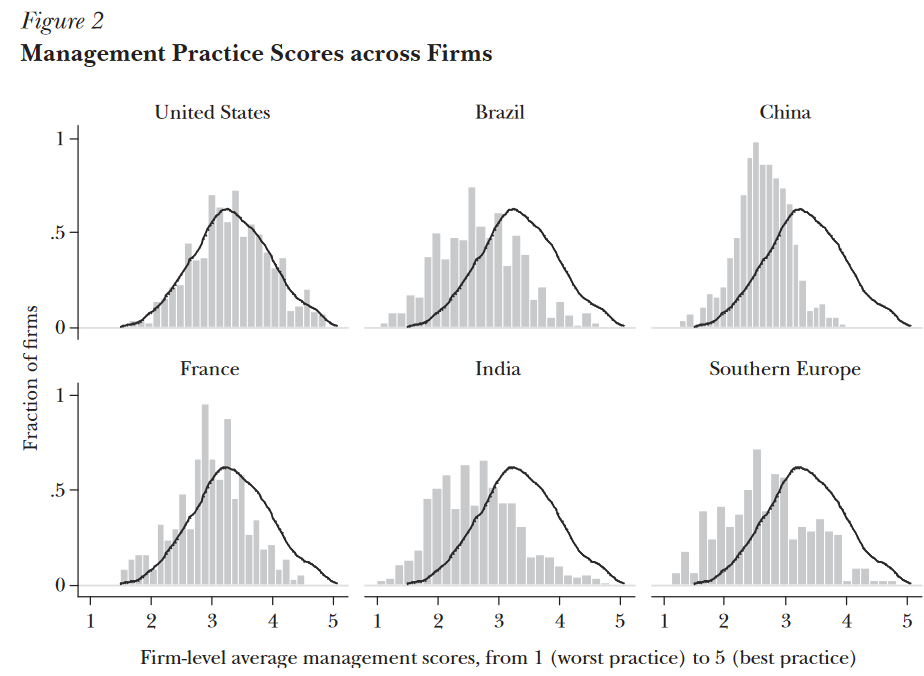
\includegraphics[width=17.4em]{pics/Bloom2010_mgmtdispersion.png}
	\label{Bloom(2010): Mgmt practices}
\end{figure}

\vspace{-1.0em}	

\begin{itemize_2pt}
	\item Heterogeneity in mgmt practices across mid-sized and large firms \citep{Bloom2007, Bloom2010, Syverson2011}
\end{itemize_2pt}
\end{frame}


\begin{frame}
\frametitle{Dispersion of Business Practices}

Public-sector companies

\begin{figure}[htbp]
	\centering
	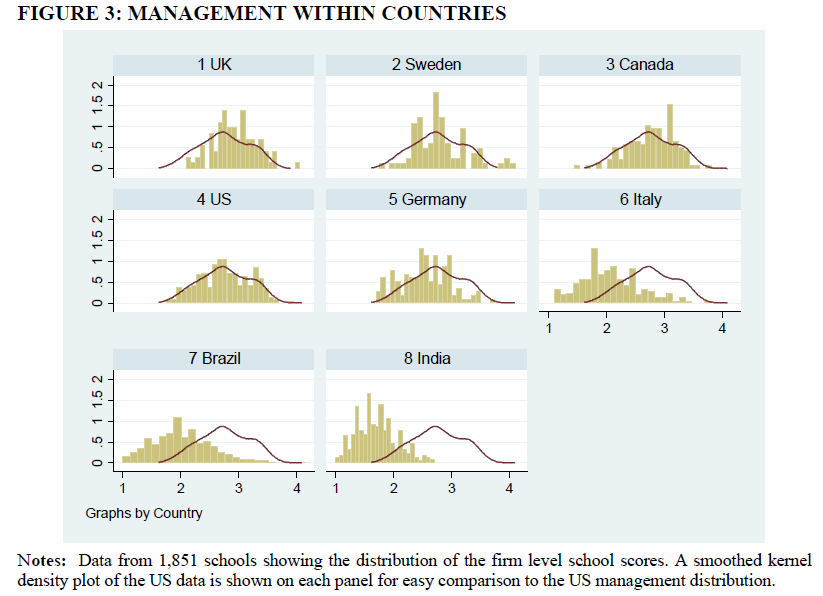
\includegraphics[width=17.4em]{pics/Bloom2015_mgmtdispersion.png}
	\label{Bloom(2015): Mgmt practices}
\end{figure}

\vspace{-1.0em}

\begin{itemize_2pt}
	\item Heterogeneity in mgmt practices across schools \citep{Bloom2015} and hospitals \citep{Bloom2020}
\end{itemize_2pt}
\end{frame}


\begin{frame}
\frametitle{Dispersion of Business Practices}

Small firms

\begin{figure}[htbp]
	\centering
	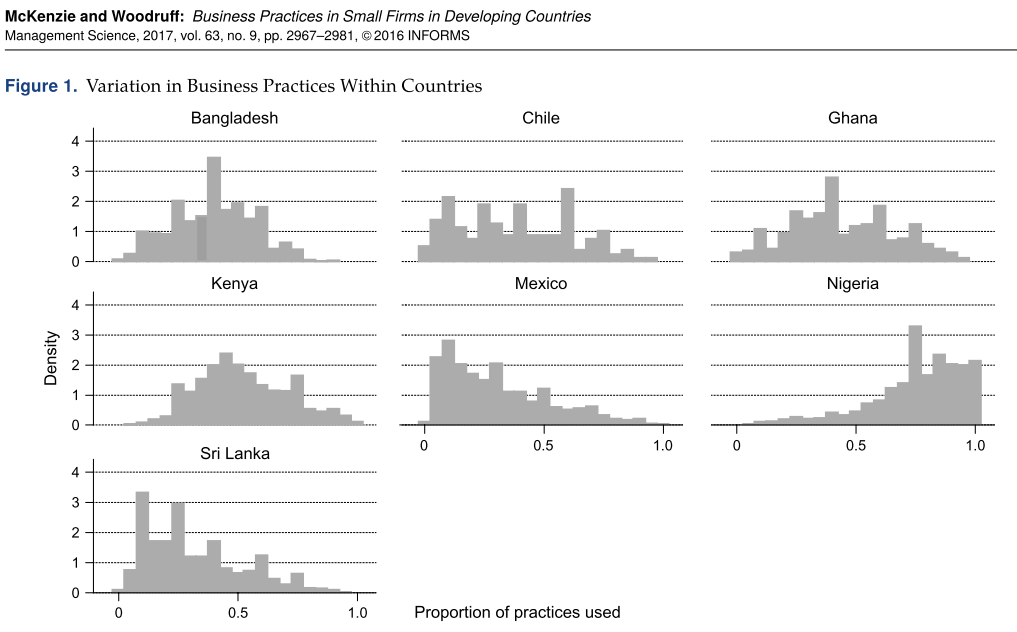
\includegraphics[width=20em]{pics/McKenzie2017_mgmtdispersion.png}
	\label{McKenzie(2017): Mgmt practices}
\end{figure}

\vspace{-1.0em}

\begin{itemize_2pt}
	\item Heterogeneity in business practices across micro and small enterprises \citep{McKenzie2017}
\end{itemize_2pt}
\end{frame}


%---------------------

\begin{frame}
\frametitle{Characterization of Business Practices}

Set of general best practices for small firms

\begin{itemize_2pt}
	\item \citet{McKenzie2017} identify set of \textcolor{bdf}{26 business practices} most closely associated with business performance
		
	\begin{itemize_2pt}	
	\vspace{0.5em}
	
		\item Validated in \textcolor{bdf}{7 countries} in Asia, Africa, and South America

		\item \textcolor{bdf}{4 major domains} of business practices
		\begin{enumerate_2pt}
			\item Book-keeping and accounting
			\item Financial planning
			\item Inventory management and stock control
			\item Marketing
		\end{enumerate_2pt}	
		
		\vspace{0.5em}	
		
		\item[] $\rightarrow$ \textcolor{bdf}{Strong persistent component} at one-year endline ($r=0.59$)
	\end{itemize_2pt}
	
	\item[] $\rightarrow$ How exactly should we think about business practices translating into performance gains?
	
\end{itemize_2pt}

\end{frame}


%\begin{frame}
%\frametitle{Characterization of Business Practices}
	
%\begin{itemize_2pt}
%	\item \citet{McKenzie2017} identify set of \textcolor{bdf}{26 business practices} most closely associated with business performance
		
%	\begin{itemize_2pt}	
%	\vspace{0.5em}
	
%		\item Example practices:
		
%		\begin{enumerate_2pt}
%			\item e.g., 
%			\item e.g., 
%			\item e.g., 
%			\item e.g.,  
%		\end{enumerate_2pt}		
		
%		\vspace{0.5em}	
		
%	\end{itemize_2pt}
	

		

	
%\end{itemize_2pt}	
	
%\end{frame}


\begin{frame}
\frametitle{Business Practices in the Production Decision}

Standard Production Decision
	\begin{itemize_2pt}
		\item Owner maximizes output $Y = f(\textcolor{red}{A}, \textcolor{bdf}{L, M, K})$ at given wealth $\textcolor{red}{W}$:	
		
		\item[] $\boxed{ \begin{aligned} \max _{\textcolor{bdf}{K, M, L}} &\{\textcolor{red}{p} \text{ } f(\textcolor{red}{A}, \textcolor{bdf}{L, M, K})-\textcolor{red}{w} \textcolor{bdf}{L}-\textcolor{red}{s} \textcolor{bdf}{M}-\textcolor{red}{r} \textcolor{bdf}{K}\} \end{aligned} }$
		\item[] $\boxed{ \begin{aligned} \text{s.t.} &\ \textcolor{red}{w} \textcolor{bdf}{L}+\textcolor{red}{s} \textcolor{bdf}{M}+\textcolor{red}{r} \textcolor{bdf}{K} \leq \textcolor{red}{\lambda} \textcolor{red}{W} \end{aligned} }$
		
		\vspace{0.5em}		
		
		\begin{itemize_2pt}
			\item[] .. where $\textcolor{bdf}{L}$ is labor, $\textcolor{bdf}{M}$ is materials, and $\textcolor{bdf}{K}$ is capital.
			\item[] .. where $\textcolor{red}{w}$ the cost of labor, $\textcolor{red}{s}$ the cost of raw materials, $\textcolor{red}{r}$ cost of capital, and $\textcolor{red}{p}$ is the output price
			\item[] .. where $\textcolor{red}{A}$ represents a productivity factor and \textcolor{red}{$\lambda$} parameterizes borrowing constraints
		\end{itemize_2pt}	
		
		\pause
		
		\vspace{0.5em}	
		
		\item 2 general conceptualizations of business practices
		\begin{enumerate_2pt}
			\item As factor of production $\textcolor{bdf}{B}$ chosen by owner at market price $\textcolor{red}{p_{B}}$
			\item As technology affecting productivity factor $\textcolor{red}{A}$
			\item[] \citep[See, e.g.,][]{Bloom2016, McKenzie2017}
		\end{enumerate_2pt}

	\end{itemize_2pt}

\end{frame}

\begin{frame}
\frametitle{Business Practices in the Production Decision}

\begin{itemize_2pt}

	\item \normalsize Further specific channels of potential impact
	\begin{enumerate_2pt}
		\item Better \textcolor{bdf}{negotiation practices} may affect raw material prices $\textcolor{red}{s}$
		\item \textcolor{bdf}{Record-keeping} and \textcolor{bdf}{financial planning practices} may affect borrowing constraints $\textcolor{red}{\lambda}$ through banks' willingness to lend \citep[see, e.g.][]{Bruhn2013}
		\item \textcolor{bdf}{Marketing practices} may affect output price $\textcolor{red}{p}$ by changing demand

\vspace{1.0em}

		\item[] $\rightarrow$ Plausible association between business practices and revenues, profits, and business growth
		
\vspace{0.5em}		
		
		\item[] $\rightarrow$ Prices ($\textcolor{red}{p}$, $\textcolor{red}{s}$, and $\textcolor{red}{p_{B}}$) and inputs ($\textcolor{bdf}{K}$, $\textcolor{bdf}{L}$, and $\textcolor{bdf}{M}$) likely endogenous to business practices $\textcolor{bdf}{B}$
	\end{enumerate_2pt}
\end{itemize_2pt}

\end{frame}



\begin{frame}
\frametitle{Business Practices and Performance}

	Using panel data and a model that treats managerial capital as technology, \citet{Bloom2016} find differences in management practices account for about 30\% of cross-country TFP differences
	\begin{itemize_2pt}
		\item Robust correlation with productivity in \textcolor{bdf}{mid-sized and large firms}, and in the \textcolor{bdf}{public sector} \citep{Bloom2015,Bloom2020} %\citep{Bloom2019}
		\item Robust correlation with performance and firm survival across industries and contexts in \textcolor{bdf}{small firms} \citep{McKenzie2017}
		\end{itemize_2pt}
		
\vspace{0.1in}	
	
	Open questions
	\begin{itemize_2pt}
		\item Does adoption of best practices \emph{cause} performance to increase?
		\item How can adoption of practices best be encouraged?
	\end{itemize_2pt}	
	
\end{frame}


\subsection{Classical MSME Training}

\begin{frame}
\frametitle{History and Prevalence}
	\begin{itemize_2pt}
		\item At least \textcolor{bdf}{USD 1 billion per year} \citep[for $\sim$ 4-5 million entrepreneurs;][]{McKenzie2021}
		\item Classical training programs \emph{precede} evidence that business practices vary and are predictive for productivity
		
		\vspace{0.5em}		
		
		\item Examples:
		\begin{itemize_2pt}
			\item Start and Improve Your Business (ILO)
			\item Business Edge (IFC)
			\item EMPRETEC Entrepreneurship Training Workshop (UNCTAD)
		\end{itemize_2pt} 
	\end{itemize_2pt}
\end{frame}

%----------------------

\begin{frame}
\frametitle{Typical Training Program}
Stylized facts on MSME trainings
\begin{itemize_2pt}
	\item Group of 15 to 40 entrepreneurs per trainer
	\item \textcolor{bdf}{In-class} (may incl elements of active and interactive learning)
	\item Period of up to two weeks	
	\item Foci of typical syllabi
	\begin{itemize_2pt}
		\item \textcolor{bdf}{Encourage start-up}: Business ideas and business plans, permits, costing, pricing, and budgeting
		\item \textcolor{bdf}{Grow existing businesses}: Record-keeping, accounting, and financial planning, marketing, human resources and hiring, stock and inventory management
	\end{itemize_2pt}
	
	\item Average training program not inexpensive \citep[USD 177 per person for ILO training;][]{vanLieshout2017}
	\item[] $\rightarrow$ Typical training program \textcolor{bdf}{highly subsidized}
	\item[] \quad (Median contribution 10\% of full price)
	
\end{itemize_2pt}

\end{frame}


\begin{frame}
\frametitle{Typical Training Program}
	
Demand for business training
	
\begin{figure}[htbp]
	\centering
	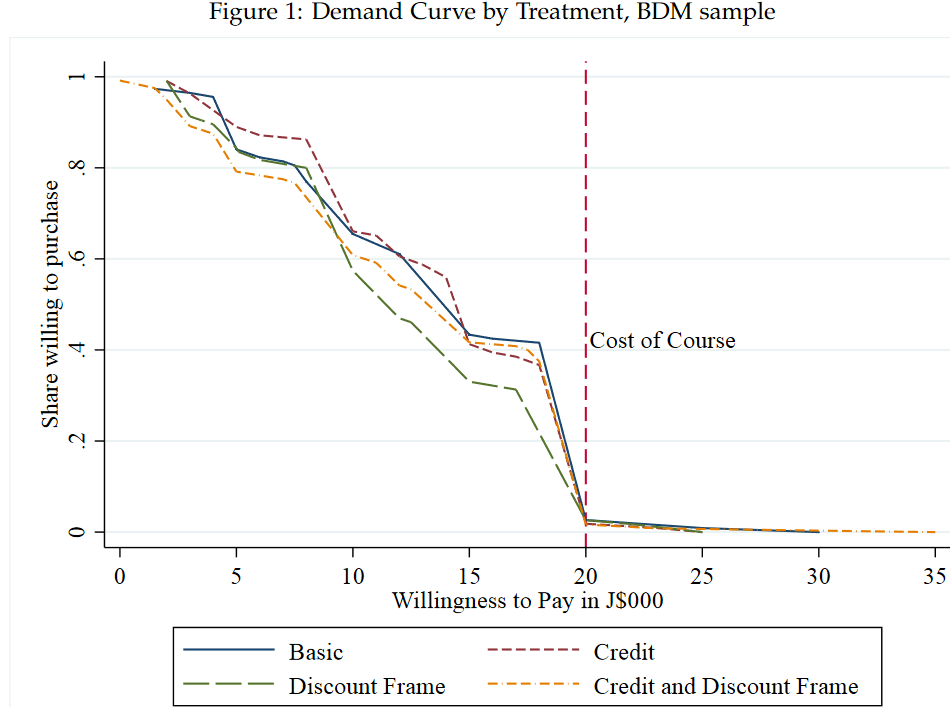
\includegraphics[width=17em]{pics/Maffioli2020_demand.png}
	\label{Maffioli(2020): Demand}
\end{figure}

\begin{itemize_2pt}
	\item Demand curve for business training in Jamaica: \textcolor{bdf}{$\sim$10\% willing to pay full price}, $\sim$60-70\% half  \citep{Maffioli2020}
\end{itemize_2pt}

\end{frame}

%---------------------

\begin{frame}
\frametitle{Impact on Performance}
First wave of evaluations
	\begin{itemize_2pt}
	\item  Headline result: \textcolor{bdf}{No impact on business performance}
	\begin{itemize_2pt}
		\item Modest short-term adoption of practices (long-term fade-out)
		\item Null-effect on business sales and profits
		\item Early examples: \citet{Field2010, Karlan2011, Bruhn2013}; also \citet[][WP in 2014]{Gine2021} 
	
	\end{itemize_2pt}
\end{itemize_2pt}
\end{frame}

\begin{frame}
\frametitle{Impact on Performance}

Econometric and implementation issues \citep{McKenzie2014}
	\begin{itemize_2pt}
		\item \textcolor{bdf}{Lack of statistical power} with MDEs often substantially above policy-relevant levels
		\begin{itemize_2pt}	
			\item Small samples (typically $N=200-400$ per treatment cell)
			\item Typical attendance between 40 and 70\%
			\item Often substantial rates of survey attrition (up to $24-28\%$)
			\item Large heterogeneity in age, education, training delivery and costs, etc.
		\end{itemize_2pt}
		
		\pause
		
		\item \textcolor{bdf}{Endline follow-ups typically short-term} (typically 1-2 years out)
		
		\item Sources of \textcolor{bdf}{selection bias} by treatment status
		\begin{itemize_2pt}	
			\item Firm survival can be endogenous on treatment
			\item Record-keeping likely to increase reporting accuracy
			\item Clear potential for differential experimenter demand effects
		\end{itemize_2pt}
		
		\item Most trainings offered at \textcolor{bdf}{no private costs}
		\begin{itemize_2pt}
			\item Potentially lower valuation, utilization \citep[see,][]{Maffioli2020}
		\end{itemize_2pt}
		
		%\item Focus on \textcolor{bdf}{existing businesses} and \textcolor{bdf}{middle-aged entrepreneurs} (typical age 35 to 45 years)
	
	\end{itemize_2pt}
\end{frame}

\begin{frame}[label=McK2020_profits]
\frametitle{Impact on Performance}
	
	Recent meta-study \citep{McKenzie2021}
	
\vspace{-0.5em}	
	
	\begin{figure}[htbp]
		\centering
		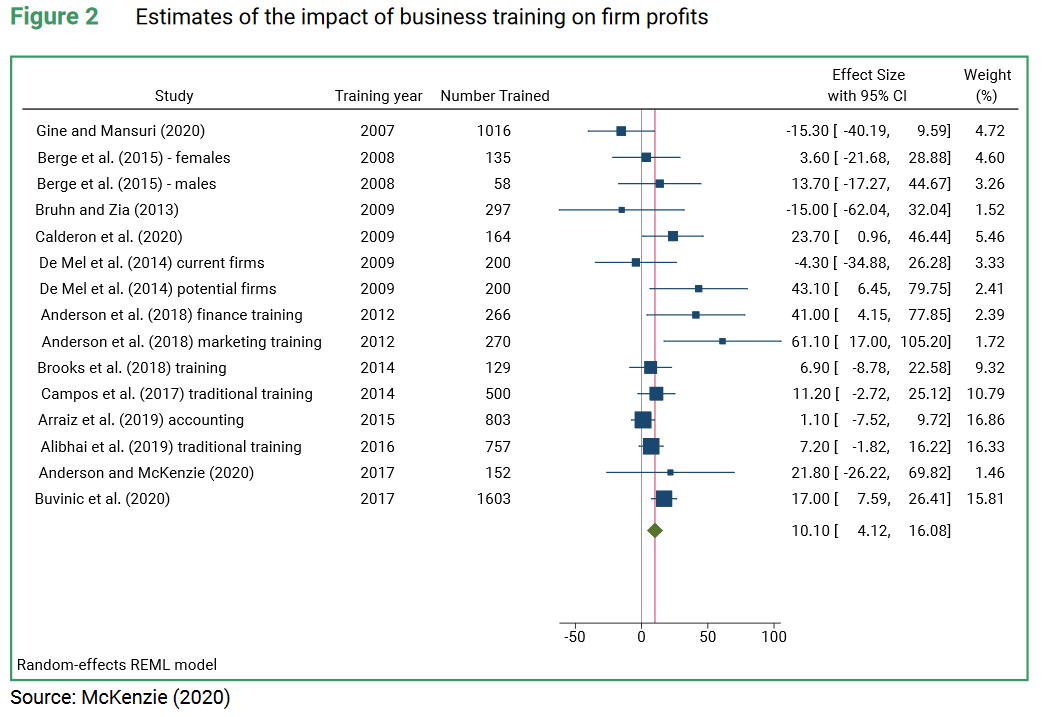
\includegraphics[width=20em]{pics/McK2020_profits.png}
		\label{McKenzie(2020): Profits}
	\end{figure}	
	
	\vspace{-1em}	
	
	\begin{itemize_2pt}
		\item \textcolor{bdf}{Small positive impact} on practice adoption and performance 
		\item[] $\rightarrow$ Estimated 10.1\% plus in profits, and 4.7\% plus in \hyperlink{McK2020_sales}{\beamergotobutton{sales}}
	\end{itemize_2pt}
	
	%Right side pics
	%\begin{tikzpicture}[remember picture, overlay]
		%\node[shift={(-6.5em,1em)}]() at (current page.south east){%
		%\hyperlink{appendix_sales}{\beamergotobutton{Sales}}};        
	%\end{tikzpicture}
	
\end{frame}

\begin{frame}
\frametitle{Targeted Training}
	Refinements of the classical model
	
	\vspace{0.5em}
	
	\begin{itemize_2pt}
		\item Targeting \textcolor{bdf}{specific subgroups} of the population
		\begin{itemize_2pt}
			\item Alleviating \textcolor{bdf}{particularly severe constraints}
			\item[] $\rightarrow$ Marginalized or disadvantaged groups (e.g., women, youth)
			\item  Maximizing \textcolor{bdf}{treatment impact} or cost-effectiveness 
			\item[] $\rightarrow$ Promising entrepreneurs (e.g., high-growth firms)
			
			\vspace{0.5em}			
			
			\item Plus: \textcolor{bdf}{Maximizing statistical power} through homogeneity
		\end{itemize_2pt}
		
	\vspace{1.0em}		
		
		\item Training of \textcolor{bdf}{specific clusters of business practices}
		\begin{itemize_2pt}
			\item Alleviating \textcolor{bdf}{specific constraints}
			\item Investigating mechanisms of treatment impact
		\end{itemize_2pt}
	\end{itemize_2pt}
\end{frame}

\begin{frame}
\frametitle{Targeted Training}
	Female entrepreneurs
	\begin{itemize_2pt}
		\item Examples: 
		\begin{itemize_2pt}
			\item Gender and Enterprise Together \citep[GET Ahead, ILO;][]{Bulte2017, McKenziePuerto2021}
			\item Start and Improve Your Business \citep[SIYB, IFC;][]{deMel2014}
		\end{itemize_2pt}
		\item \textcolor{bdf}{Most common type of targeted training} (complementary to classical microfinance model)
		
		\vspace{0.5em}
		
		\item Structural reasons
		\begin{itemize_2pt}
			\item Women overrepresented in mere subsistence entrepreneurship
			\item Female entrepreneurs often subject to more severe constraints
			\item[] \citep[e.g., due to household-level reallocation; see][]{Bernhardt2019, deMel2009a}
		\end{itemize_2pt}
	\end{itemize_2pt}
\end{frame}

\begin{frame}
\frametitle{Targeted Training}
	Young entrepreneurs
	\begin{itemize_2pt}
		\item Typically embedded as \textcolor{bdf}{entrepreneurship courses in school or university} (business concepts and soft skills)
		\item Example: Final year university course in Tunisia \citep{Alaref2020}
		\begin{itemize_2pt}
			\item Initial positive impact on business entry
			\item[] $\rightarrow$ \textcolor{bdf}{Effects taper off after 4 years} (no evidence for lasting effects)
		\end{itemize_2pt}
	\end{itemize_2pt}
	
\pause

\vspace{0.5em}

High-growth businesses ("gazelles")
\begin{itemize_2pt}
	\item Extensive-margin prediction of future MSE growth is hard \citep{Fafchamps2017}
	\begin{itemize_2pt}
		\item Survey, ability measure, expert panel all explain unique variation
		\item But: \textcolor{bdf}{Business training for predicted gazelles shows no impact}
	\end{itemize_2pt} 
	
	\item \citet{McKenzie2017a} finds \textcolor{bdf}{more encouraging results with a large-scale, high-stakes business plan competition} in Nigeria
	
	\item Small literature on business accelerators and incubators
	\begin{itemize_2pt}
		\item See, e.g., \citet{Cusolito2021, GonzalezUribe2018, GonzalezUribe2021}
	\end{itemize_2pt}
\end{itemize_2pt}
	
\end{frame}

%---------------------

\begin{frame}
\frametitle{Targeted Training}

Training of specific clusters of practices
\begin{itemize_2pt}	
	\item \citet{Anderson2018} assign 852 South African micro-entrepreneurs to distinct types of training:
	
	\vspace{0.5em}	
	
	\begin{enumerate_2pt}
		\item Marketing/sales skills
		\item[]
		\item[]
		\item[]
		\item Finance/accounting skills
		\item[]
		\item[]
		\item[]
	\end{enumerate_2pt}
\end{itemize_2pt}

\end{frame}


\begin{frame}
\frametitle{Targeted Training}

Training of specific clusters of practices
\begin{itemize_2pt}	
	\item \citet{Anderson2018} vary \textcolor{bdf}{training focus} among 852 South African micro-entrepreneurs
	
	\vspace{0.5em}	
	
	\begin{enumerate_2pt}
	
		\item Marketing/sales skills
		\begin{itemize_2pt}
			\item \textcolor{bdf}{"Growth focus" on higher sales, stock investments, and hiring}
			\item 61\% increase in profits
			\item[] $\rightarrow$ Benefits new businesses ($=$ less market exposure)
		\end{itemize_2pt}		
		
		\item Finance/accounting skills
		
		\pause		
		
		\begin{itemize_2pt}
			\item \textcolor{bdf}{"Efficiency focus" on lower costs}
			\item 41\% increase in profits
			\item[] $\rightarrow$ Benefits established businesses
		\end{itemize_2pt}
			
	\end{enumerate_2pt}
	
		\item[] $\rightarrow$ Different "pathways to profits"

\end{itemize_2pt}

\end{frame}


\subsection{Extensions of the Classical Approach}

\begin{frame}
\frametitle{On-site Consulting}

Stylized facts on business consulting
\begin{itemize_2pt}
	\item Three-step procedure
	\begin{enumerate_2pt}
		\item Diagnosing practices
		\item Identifying areas of improvement
		\item Joint and interactive problem solving
	\end{enumerate_2pt}
	
	\pause
	
	\item Typically one-on-one \citep[also group-based; see,][]{Iacovone2021}
	
	\item \textcolor{bdf}{Sustained and intensive}
	\begin{itemize_2pt}
		\item Total of 88 to 200 hours and more \citep{Anderson2020, Bruhn2018} %[citation]Karlan2015, Bruhn2019
		\item[] $\rightarrow$ Typically several months
		\item[] $\rightarrow$ Meetings monthly to twice weekly, 2-4 hours
		\item Total cost between \textcolor{bdf}{USD 4,000 and 12,000 per firm} \citep{Anderson2020, Bruhn2018}
	\end{itemize_2pt}
	
	\item \textcolor{bdf}{Often gov't-subsidized} (private contributions typically $\sim$10\%) \\
	\begin{itemize_2pt}
		\item[] $\rightarrow$ \textcolor{bdf}{Matching-grant programs}
	\end{itemize_2pt}
	
\end{itemize_2pt}
\end{frame}


\begin{frame}
\frametitle{On-site Consulting}

Example: Matching grant program for MSMEs in Mexico \citep{Bruhn2018}
\begin{itemize_2pt}

	\item Weekly 4-hour visits over one year
	\item USD 12,000 per person (subsidized at $70-90\%$)
	\item \textcolor{bdf}{Small positive impacts on profits and ROA after 1 year}
	

	\vspace{0.5em}	
	
	\item Using admin data, \textcolor{bdf}{57\% higher employment after 5 years}
	\begin{itemize_2pt}
		\item Limited availability of admin data may introduce \textcolor{bdf}{selection bias}
		\item Not clear if effects concentrated among few businesses
	\end{itemize_2pt}
\end{itemize_2pt}

\begin{figure}[htbp]
	\centering
	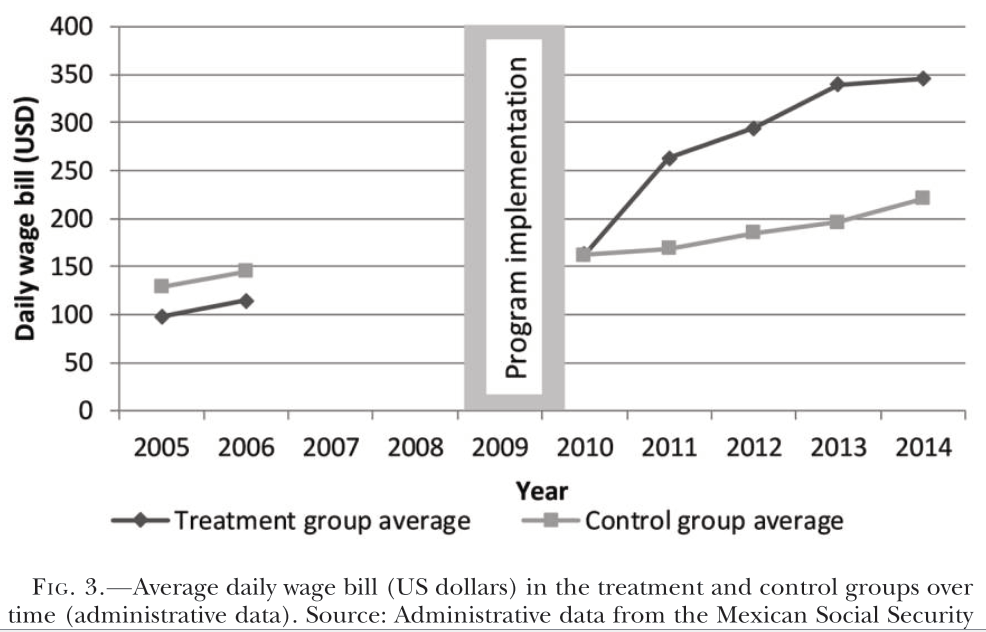
\includegraphics[width=15em]{pics/Bruhn2018_consult.png}
	\label{Bruhn (2018): Consulting}
\end{figure}


\end{frame}

%---------------------

\begin{frame}
\frametitle{Multimedia delivery}
TV shows
\begin{itemize_2pt}
	\item Examples: \textcolor{bdf}{Reality show competitions} in Tanzania \citep{Bjorvatn2020} and Egypt \citep{Barsoum2018}
	\item Differential random incentivization schemes
	\item[] $\rightarrow$ \textcolor{bdf}{No impact} on business knowledge and business entry 
	\item[] $\rightarrow$ But: \textcolor{bdf}{High viewership} (conventional MDEs substantially above policy-relevant levels) 
 
\end{itemize_2pt}

\pause
	
\vspace{0.5em}
	
Text messages
\begin{itemize_2pt}
	\item Examples: 
	\begin{itemize_2pt}
		\item Heuristics-based business advice \citep{Cole2018}
		\item Personalized inventory recommendations \citep{Acimovic2020}
	\end{itemize_2pt}
	\item[] $\rightarrow$ Small literature with generally \textcolor{bdf}{mixed results or null effects}
	\item[] $\rightarrow$ But: \textcolor{bdf}{Extremely cheap} (MDEs above policy-relevant levels)
	\item[] $\rightarrow$ But: \textcolor{bdf}{Potential complementarities} with in-person training
\end{itemize_2pt}
\end{frame}

% -----------------------


%\begin{frame}
%\frametitle{Complementary Constraints}
%	\begin{itemize_2pt}
%	\item Core idea: \textcolor{bdf}{Address multiple interrelated constraints}
%	\item Examples: de Mel et al. (2014), Berge et al. (2015), Gine and Iacovone (2021)
%	\end{itemize_2pt}
%\end{frame}


\subsection{Measuring Firm Performance}

\begin{frame}
\frametitle{Variation in Outcome Measures}
	
	\begin{figure}[htbp]
		\centering
		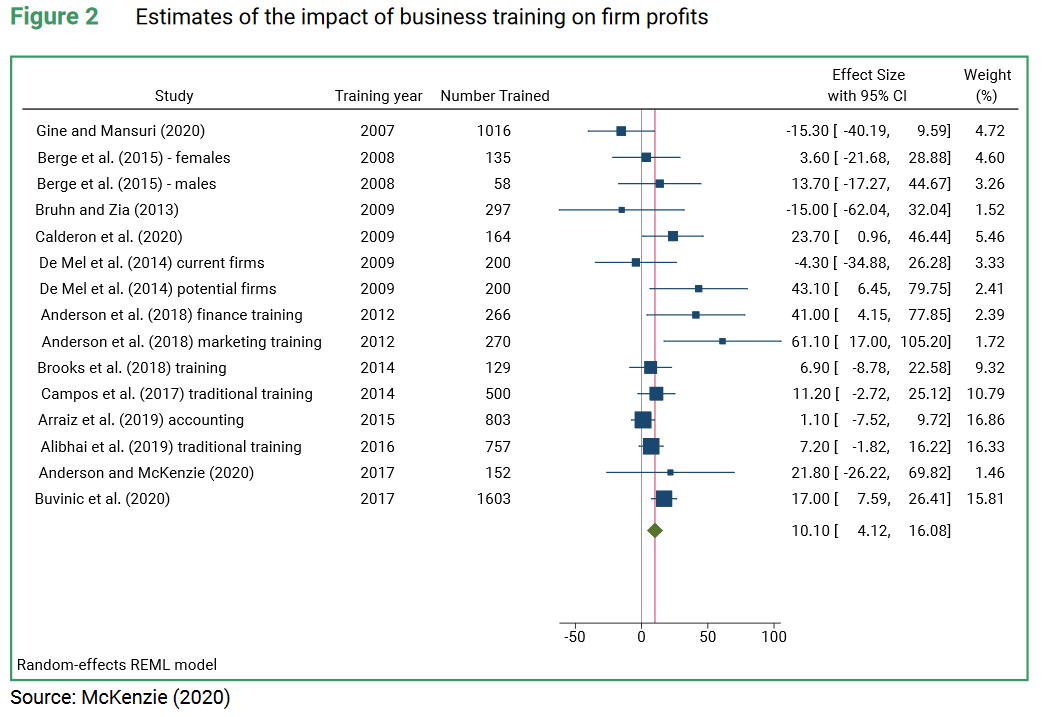
\includegraphics[width=23.5em]{pics/McK2020_profits.png}
		\label{McKenzie(2020): Profits2}
	\end{figure}	
	
\vspace{-1em}	
	
	\begin{itemize_2pt}
		\item \textcolor{bdf}{Extremely wide confidence intervals} on impact estimates
	\end{itemize_2pt}
\end{frame}


\begin{frame}
\frametitle{Variation in Outcome Measures}

Alternative measures of business profits \citep{deMel2009}
	\begin{itemize_2pt}
		\item 15-16 unannounced visits during one month
		\item Random assignment of profit measure, accounting diaries, and recall span
	\end{itemize_2pt}
		
	\pause	
		
	\vspace{0.5em}
		
	\begin{enumerate_2pt}
		\item \textcolor{bdf}{Self-reported profits most accurate measure}
		\item[] $\rightarrow$ Correlation with sales-minus-expenditures only $r=0.3$
		\item \textcolor{bdf}{Accounting diaries have no effect on profits} (but on sales)
		\item With recall over 4 months vs. 1 month, entrepreneurs \textcolor{bdf}{understate revenues by $10 - 15 \%$ due to memory loss} 
		\item Entrepreneurs estimate average rival business to \textcolor{bdf}{underreport sales by 30\%}
	\end{enumerate_2pt}	

\end{frame}


\begin{frame}
\frametitle{Variation in Outcome Measures}

Survey media and frequencies \citep{Garlick2019}
\begin{itemize_2pt}
	\item 12-week panel with detailed measurements of employees, assets, profits, sales, transfers, etc.
	\item Random assignment to different survey modes and frequencies
	\begin{enumerate_2pt}
		\item Monthly in-person
		\item Weekly in-person
		\item Weekly phone
	\end{enumerate_2pt}
		
	\pause		
	
	\item Survey medium
	\begin{itemize_2pt}
		\item \textcolor{bdf}{All survey modes generally result in similar statistical moments}
		\item Phone surveys yield higher within-firm variation
		\item[] (And may be more vulnerable to social desirability bias.)
	\end{itemize_2pt}
	
	\item Survey frequency
	\begin{itemize_2pt}
		\item \textcolor{bdf}{Higher frequency generally does not alter statistical moments}
		\item No evidence for higher attrition
	\end{itemize_2pt}
\end{itemize_2pt}
\end{frame}


%\begin{frame}
%\frametitle{Variation in Outcome Measures}
%	\begin{itemize_2pt}
%		\item \citep{deMel2009}
%		\item \citep{Bernhardt2019}
%	\end{itemize_2pt}
%\end{frame}

%\begin{frame}
%\frametitle{Self-reports and aggregation}
%	\begin{itemize_2pt}
%	\item Direct measures \citep{deMel2009}
%	\vspace{0.1in}
%	\end{itemize_2pt}
%\end{frame}

%---------------------

\begin{frame}
\frametitle{Variation in Outcome Measures}
Technological aids \citep{Fafchamps2012}
	\begin{itemize_2pt}
	\item Random assignment to Personalized Digital Assistants (PDAs)
	\item Potential channels of impact
	\begin{enumerate_2pt}
		\item More timely data entry
		\item Greater accuracy (especially by correct use of skip patterns)
		\item More and more complex consistency checks
	
	\end{enumerate_2pt}
	
	\vspace{0.5em}	
	
	\item Key result: \textcolor{bdf}{Vast majority of large changes in sales and profits genuine income volatility}
	\begin{itemize_2pt}
		\item Positive, but limited, effect of consistency checks in reducing variation in firm performance
	\end{itemize_2pt}	
	
\end{itemize_2pt}
\end{frame}


\subsection{Mechanisms}

\begin{frame}
\frametitle{Heterogeneity of Impact}

Heterogeneity of treatment effects poorly understood across different approaches
\begin{itemize_2pt}
	\item Potential constraints are manifold, and likely context-dependent
	
\vspace{0.5em}	
	
	\item Some more obvious constraints:
	\begin{itemize_2pt}
		\item \textcolor{bdf}{Credit constraints} \citep[e.g.,][]{Berge2015, Gine2021}%[citation] mcenzie
		\item \textcolor{bdf}{Education} and \textcolor{bdf}{literacy constraints}
		\item \textcolor{bdf}{Gender norms and constraints}
		%\item \textcolor{bdf}{Age-related} network and knowledge/skill \textcolor{bdf}{constraints}
	\end{itemize_2pt} 
	
	\vspace{1.0em}

	$\rightarrow$ More recent literature highlights additional \textcolor{bdf}{behavioral constraints}	
	
\end{itemize_2pt}
	

\end{frame}

\begin{frame}
\frametitle{Education and literacy}

Most MSE entrepreneurs have limited education

\vspace{-1.9em}

\begin{figure}[htbp]
	\centering
	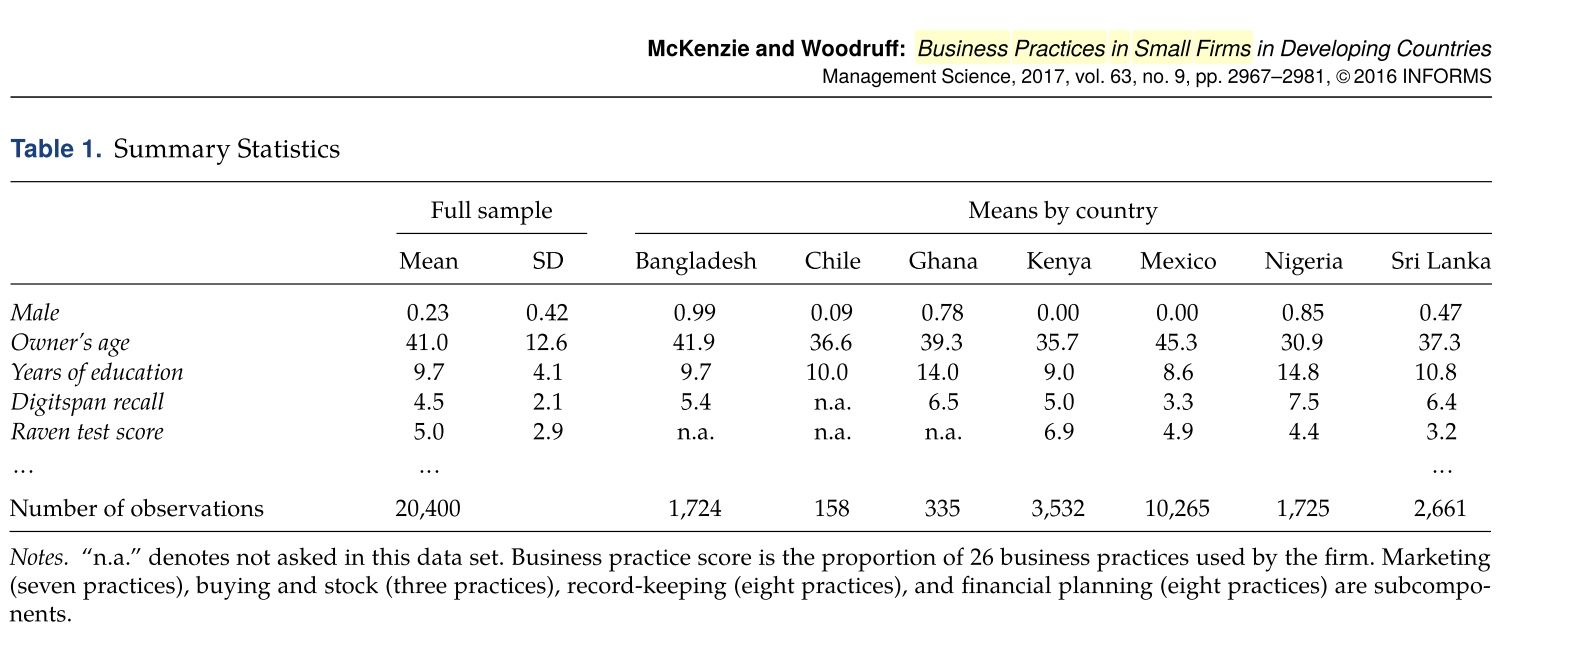
\includegraphics[width=27em]{pics/McK2017_educ.png}
	\label{McKenzie(2017): Education and cognitive functioning}
\end{figure}

\vspace{-2.5em}

\begin{itemize_2pt}
	\item Typical micro-entrepreneur is a high-school dropout
	\item Test scores on digitspan and Raven's matrices about \% of Western university samples \textcolor{red}{\citep[comp.][]{}}
\end{itemize_2pt}
\end{frame}

\begin{frame}
\frametitle{Education and literacy}

Potential for heuristics and rules of thumb
\begin{itemize_2pt}
	\item Example: Heuristics-based business training program by \citet{Drexler2014}
	\item[] $\rightarrow$ Discussed under \hyperlink{Drexler_thumb}{\beamergotobutton{alternative approaches}}
	\item See also, \citet{Cole2018} and \citet{Arraiz2019}
\end{itemize_2pt}
\end{frame}


\begin{frame}
\frametitle{Family and neighborhood}

Family commitments
\begin{itemize_2pt}
	\item \textcolor{bdf}{Unequal responsibilities for child care} \citep{Delecourt2021}
	\begin{itemize_2pt}
		\item Audit study with mystery shoppers among drug stores in Uganda
		\item Average gender profit gap of 60\%
		\item Close to all women have $\geq$ 1 child, breastfeed for median 19.8 months
		\item[] $\rightarrow$ Among female entrepreneurs, those with child at work ..
		\begin{itemize_2pt}
			\item .. are \textcolor{bdf}{out of stock} more often, and stock up less.
			\item .. have \textcolor{bdf}{48\% lower profits}.
		\end{itemize_2pt}
	\end{itemize_2pt}
\end{itemize_2pt}

\pause
\vspace{1.0em}

Market segregation
\begin{itemize_2pt}
	\item Markets can be geographically (and socially) segregated, especially in residential areas
	\begin{itemize_2pt}
		\item Potential \textcolor{bdf}{demand constraints} \citep[in the spirit of][studying women in Ghana]{Hardy2020}
		\item (Scant work, but seems important.)
	\end{itemize_2pt}
\end{itemize_2pt}
\end{frame}


\begin{frame}
\frametitle{Dynamic complementarities in skill acquisition}

Complementarities in skills
\begin{itemize_2pt}
	\item Clusters of skills may be more valuable in combination
	\begin{itemize_2pt}
		\item Record keeping and financial planning complement each other
	\end{itemize_2pt}
	\item Skills may build on each other
	\begin{itemize_2pt}
		\item Profit calculation relies on record keeping
		\item Advanced inventory management relies on record keeping (and profit calculation)
	\end{itemize_2pt}
\end{itemize_2pt}

\vspace{1.0em}

Learning styles
\begin{itemize_2pt}
	\item Exploration-exploitation trade-off 
	\begin{itemize_2pt}
		
		\item Not clear how much to exploit available best practice, and how much to invest in search for innovation
		\item Psychological research finds interpersonal differences in \textcolor{bdf}{preference for information search} \cite[see, e.g.,][]{Hills2015, Schulz2020, Gonzalez2011}
		%\item Evidence for trait-like persistence of this preference (see, e.g.,\textcolor{camel}{Waldner et al., 1998, Engler et al., 2010})%[citation]
		\item If technology has initial fixed costs, poverty \textit{per se} may affect trade-off
	\end{itemize_2pt}
	
\end{itemize_2pt}

\end{frame}


\begin{frame}
\frametitle{Aspirations}

Aspirations theory \citep[following][]{Dalton2016}
\begin{itemize_2pt}
	\item Aspirations are \textcolor{bdf}{desired level of outcome}	
	
	\item In theoretical work, aspirations are modeled as \textcolor{bdf}{reference-dependent preferences}
	\begin{itemize_2pt}
		\item Agent derives utility from relative level wrt aspirations
		\item[] $\rightarrow$ Aspirations motivate effort
		\item Behavioral constraint: \textcolor{bdf}{Agent neglects outcomes $\rightarrow$ aspirations}
	\end{itemize_2pt}
	
	\vspace{0.5em}
	
	\begin{figure}[htbp]
		\centering
		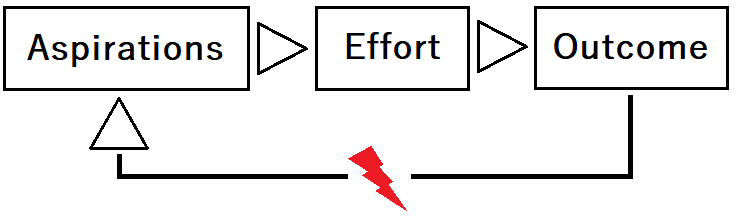
\includegraphics[width=12em]{pics/asp.png}
		\label{Aspirations}
	\end{figure}	
	
	\pause
	
	\item Consequence: Sufficiently \textcolor{bdf}{poor agents} with sufficiently \textcolor{bdf}{low aspirations} choose suboptimally low effort
	\item[] $\rightarrow$ Potential for \textcolor{bdf}{behavioral poverty trap}
	\vspace{0.1in}
	
%\begin{figure}[htbp]
%	\centering
%	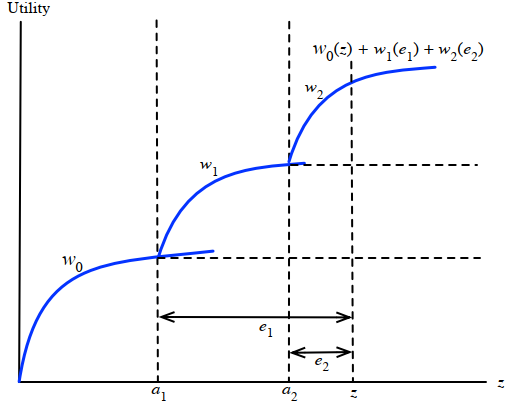
\includegraphics[width=15em]{pics/Ray2019_aspsMulti.png}
%	\label{Ray(2019): Aspirations}
%\end{figure}	
	
\end{itemize_2pt}
\end{frame}

\begin{frame}
\frametitle{Aspirations}

Evidence on aspirations in entrepreneurship
\begin{itemize_2pt}
	\item Descriptive evidence that \textcolor{bdf}{micro-entrepreneurs show sizable growth aspirations} \citep{Dalton2018}
	\begin{itemize_2pt}
		\item Both short-term and long-term, for growth in size, labor, and sales
		\item Entrepreneurs update dynamically given new information
	\end{itemize_2pt}
	
	\pause
	
	\item \href{https://www.poverty-action.org/study/impact-cash-transfers-aspirations-and-goal-setting-economic-outcomes-and-well-being}{Garlick et al. (in progress)} cross-randomize role-model intervention and large UCT to study complementarity
	\begin{itemize_2pt}
		\item \textcolor{bdf}{Exposure to role models increases aspirations, labor supply, expenditures, and sales}
		\item[] (Cash also increases aspirations, labor supply, expenditures, and sales.)
	\end{itemize_2pt}
	
	\pause
	
	\item \textcolor{bdf}{Aspiration interventions can backfire}
	\begin{itemize_2pt}
		\item Goal setting intervention resulted in \textit{lower} investment \citep{McKenzie2021a}
		\item[] $\rightarrow$ Potential of aspiration frustration if external constraints bind 
		\item[] \quad \citep[see also,][]{Galiani2018}
	\end{itemize_2pt}

\end{itemize_2pt}
\end{frame}


\subsection{Alternative Approaches}

\begin{frame}[label=Drexler_thumb]
\frametitle{Rules of Thumb}

Core idea: Provide \textcolor{bdf}{simplified rules} to make training more cognitively accessible

\begin{itemize_2pt}
	
	\item Example: 
	\begin{itemize_2pt}
		\item Instead of detailed accounting practices, ..
		\item[] .. focus on \textcolor{bdf}{physical separation of household and business finances} 
		\item[] .. and only transfer money with an explicit \textcolor{bdf}{"IOU" note}
	\end{itemize_2pt}
	
	\vspace{1.0em}
	
	\item Classical study: \citet{Drexler2014}
	\begin{itemize_2pt}
		\item Comparison of heuristics-based and standard accounting training with 1,193 micro-entrepreneurs in the Dominican  Republic
		\item Null effect for full sample
		\item[] $\rightarrow$ Statistical power limited due to substantial missing sales data
		\item[] $\rightarrow$ \textcolor{bdf}{Larger gains with heuristics-based training for less educated entrepreneurs}
		
	\end{itemize_2pt}
\end{itemize_2pt}
\end{frame}

\begin{frame}
\frametitle{Rules of Thumb}
	\begin{itemize_2pt}
		\item \citet{Arraiz2019} compare 4-hours heuristics-based finance training with standard finance and accounting program among 2,408 micro-entrepreneurs in Ecuador 
		\begin{itemize_2pt}
			\item Heuristics-based training increases daily business sales and profits by about 8\% each
			\item Effects driven by \textcolor{bdf}{women} and entrepreneurs with \textcolor{bdf}{lower cognitive scores}
		\end{itemize_2pt}
		
		\vspace{1.0em}
		
		\item Points of critique
		\begin{itemize_2pt}
			\item \textcolor{bdf}{Limited target group} of cognitively challenged
			\item \textcolor{bdf}{Limited scope} (mostly confined to accounting practices)
			\item So far \textcolor{bdf}{no long-term follow-up} (studies use 1-year endlines)
			\item \citet{Cole2018} find more mixed evidence for text-based rule-of-thumb assistance among micro-entrepreneurs in India and The Philippines
		\end{itemize_2pt}
		
	\end{itemize_2pt}
\end{frame}

%

\begin{frame}
\frametitle{Entrepreneurial mindset}

Core idea: \textcolor{bdf}{Develop proactive mindset and increase growth aspirations}
\begin{itemize_2pt}
	\item Examples: 
	\begin{itemize_2pt}
		\item Encourage continued search for new opportunities
		\item Encourage reflection on business differentiation
		\item Learning by doing and from mistakes
		\item Set daily goals
	\end{itemize_2pt}
	
	\vspace{1.0em}
	
	\item \citet{Campos2017} compare mindset training to standard business training among 1,500 micro-entrepreneurs in Togo
	\begin{itemize_2pt}
		\item 36 hours classroom instruction
		\item 4 monthly 3-hours one-on-one follow-ups by trainer
		\item USD 750 per person
		\item[] $\rightarrow$ \textcolor{bdf}{Initiative training improves business profits by 30\% over 2.5 years}
		\item[] \quad (Standard business training improves profits by 11\%)
		\item[] $\rightarrow$ \textcolor{bdf}{Costs amortized within a year through firm profits}
	\end{itemize_2pt}

	\end{itemize_2pt}
\end{frame}

\begin{frame}
\frametitle{Entrepreneurial mindset}

\begin{figure}[htbp]
	\centering
	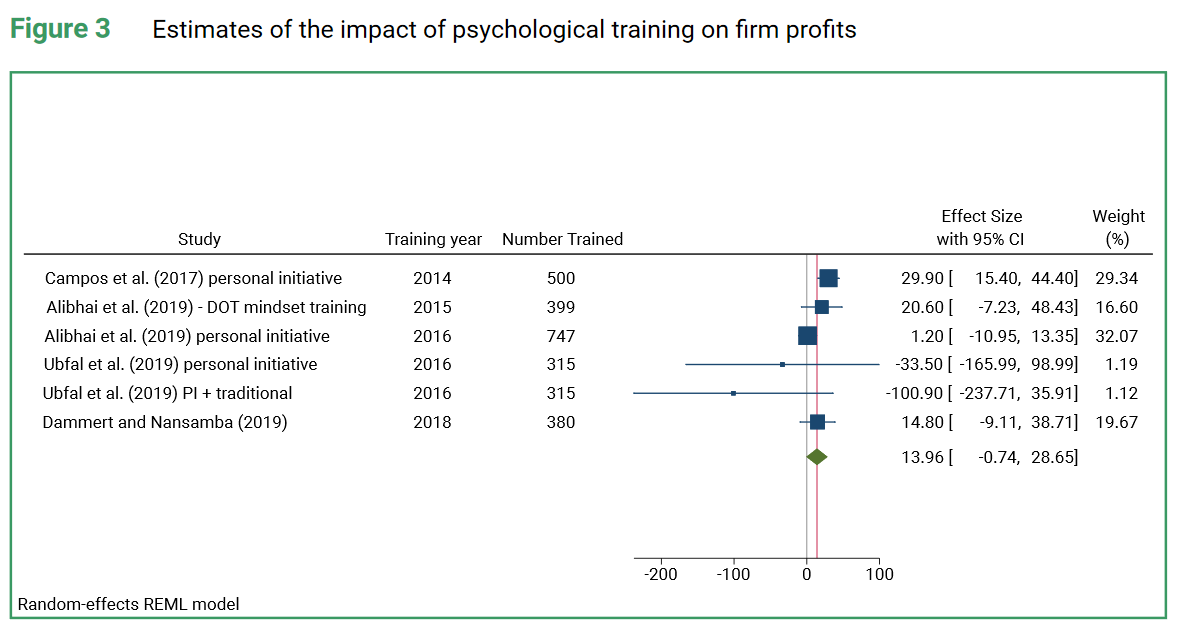
\includegraphics[width=23em]{pics/McKenzie2020_mindset.png}
	\label{McKenzie (2020): Mindset}
\end{figure}

\vspace{-1.0em}

\begin{itemize_2pt}
	\item \textcolor{bdf}{Average increases in business profits of 14\% and in sales of 10\%}
	\item Programs show \textcolor{bdf}{substantial heterogeneity} wrt content and focus
	\item[] $\rightarrow$ Heterogeneous, but generally positive, results
\end{itemize_2pt}
\end{frame}

\begin{frame}
\frametitle{Entrepreneurial mindset}

Points of critique
\begin{itemize_2pt}
	\item \textcolor{bdf}{Probably limited target group}
	\item Not clear whether standard curriculum and personal initiative training are \textcolor{bdf}{complements or substitutes}
	\item \citet{Alibhai2019} and \citet{Ubfal2020} find \textcolor{bdf}{mixed results with lower treatment intensity}
	\item No work yet on whether \textcolor{bdf}{classroom training and/or one-on-one follow-ups} necessary and/or sufficient conditions for success
\end{itemize_2pt}
\end{frame}

%---------------------

\begin{frame}
\frametitle{Local Knowledge and Mentoring}

Local entrepreneurs as mentors

\begin{itemize_2pt}

	\item Core ideas: 
	\begin{itemize_2pt}
		\item \textcolor{bdf}{Information may be highly localized}
		\item \textcolor{bdf}{Peers may know better} about particular local constraints and practices
		\item \textcolor{bdf}{Social learning} may work better between peers
		\item Local mentors may be more \textcolor{bdf}{cost effective}
	\end{itemize_2pt}
	
	\item[] $\rightarrow$ Who mentors?
	\item[] $\rightarrow$ Will mentors agree to share information?
	\item[] $\rightarrow$ How to incentivize continued mentoring?
		
\end{itemize_2pt}
\end{frame}

\begin{frame}
\frametitle{Local Knowledge and Mentoring}

\begin{itemize_2pt}
	\item Successful business owners mentor smaller firms \citep{Brooks2018}
	\begin{itemize_2pt}
		\item Random assignment of mentors or standard business training to 372 female micro-entrepreneurs in Kenya
		\item Mentorship dyads
		\begin{itemize_2pt}
			\item Mentors local entrepreneurs from more profitable firms
			\item \textcolor{bdf}{Encouragement of weekly meetings at mentor's firm for one month}
			\item Many dyads continue meeting for more than one year
		\end{itemize_2pt}
		
		\item Mentored businesses show \textcolor{bdf}{increases in profits by 20\%}
		\item $\rightarrow$ \textcolor{bdf}{Effect fades after one year} (when dyad dissolves)
		\item No effect of standard business training.
		
		\vspace{0.5em}
		
		\item \citet{McKenziePuerto2021} find no impact of a 5-months mentoring scheme among female micro-entrepreneurs in Kenya
	\end{itemize_2pt}
\end{itemize_2pt}

\end{frame}

\begin{frame}
\frametitle{Local Knowledge and Mentoring}

Peer-to-peer learning

\begin{itemize_2pt}
	\item Core idea: \textcolor{bdf}{Firms may improve through mutual social learning}
	
	\vspace{0.5em}
	
	\item Firms matched among peers \citep{Cai2018}
	\begin{itemize_2pt}
		\item Random assignment of \textcolor{bdf}{peer group meetings} among 2,820 SMEs in China
		\item Monthly meetings with 9 peers for 10 months
		\item Peer groups of different sizes and sector compositions
		
		\vspace{0.5em}
		
		\item[] $\rightarrow$ \textcolor{bdf}{Sales increased by $8-10\%$} 
		\item[] $\rightarrow$ Comparable increases in material inputs, employment, and assets

	\end{itemize_2pt}

\end{itemize_2pt}


\end{frame}

%---------------------




\addtocontents{toc}{\protect\setcounter{tocdepth}{0}}

\subsection{Takeaways}

\begin{frame}
\frametitle{Takeaways}
	\begin{itemize_2pt}
    \item \textcolor{bdf}{Business practices differ substantially across firms} ..
    \item[] \quad .. and vary with productivity
    \item \textcolor{bdf}{Standard business training has limited ability} to change practices and firm performance in the short-term ..
    \item[] \quad .. while long-term evidence is scarce
    \item Some of that is due to \textcolor{bdf}{measurement error} (especially wrt firm profits) and \textcolor{bdf}{lack of statistical power} ..
    \item[] \quad .. but \textcolor{bdf}{extensions of classical approach} also show promise:
    
\vspace{0.5em}    
    
    \begin{itemize_2pt}
    	\item Personal initiative training
    	\item Business mentoring
    	\item Peer-to-peer learning
    \end{itemize_2pt}
   	\vspace{0.10in}
\end{itemize_2pt}
\end{frame}

\begin{frame}
\frametitle{Questions}
	\textcolor{bdf}{Any questions?}
	\begin{itemize_2pt}
	\item[] .. before we move on to our paper?
	\end{itemize_2pt}
\end{frame}


%-----------------------------------------------------------
%------------------------------------------------------------
%------------------------------------------------------------
%------------------------------------------------------------
%------------------------------------------------------------

\addtocontents{toc}{\protect\setcounter{tocdepth}{99}}

\title[]{Curating Local Knowledge}
\subtitle{Experimental Evidence from Small Retailers in Indonesia}

\author[]
{Patricio S. Dalton\inst{1}\
Julius R{\"u}schenp{\"o}hler\inst{2}
Burak Uras\inst{1}\\and
Bilal Zia\inst{3}}

\institute[]{
\inst{1} Tilburg University \\
\inst{2} UC Berkeley, CEGA\\
\inst{3} The World Bank}

\date{March 04, 2021}


\section{\textbf{PART II: Paper} \\ \quad \emph{Curating Local Knowledge}}

\setbeamertemplate{sidebar right}{}

\begin{frame}
\titlepage
\end{frame}


\setbeamertemplate{sidebar right}[sidebar theme]

\begin{frame}{Paper Overview}
\tableofcontents[currentsection,hideothersubsections]
\end{frame}


%------------------------------------------------
\subsection{Motivation}

\begin{frame}
\frametitle{Background}
	\begin{itemize_2pt}
	\item Micro and small firms (MSEs) are typically the main \textcolor{bdf}{source of employment} in the developing world
	\item In \textcolor{bdf}{Indonesia}, MSEs represent .. 
	\begin{itemize_2pt}
		\item .. 99\% of all firms
		\item .. 94.5\% of employment
	\end{itemize_2pt} 
	\item Understanding the factors fostering efficiency and growth of MSEs is an important research and policy goal
	\end{itemize_2pt}
\end{frame}

%------------------------------------------------
\begin{frame}
\frametitle{A Growing Focus on Management}
\begin{itemize_2pt}
\item \textcolor{bdf}{Classroom Training}: \citet{McKenzie2014, Karlan2011, Bruhn2013, Anderson2018, Bulte2017, Field2010}
\vspace{0.1in}
\item \textcolor{bdf}{Consulting}:\citet{Bruhn2018, Anderson2020, Karlan2015}
\vspace{0.1in}

\item \textcolor{bdf}{Mobilizing Peer Knowledge}:
    \begin{itemize_2pt}
    \item \citet{Brooks2018} $\rightarrow$ Local mentors (market information)
    \item \citet{Cai2018} $\rightarrow$ Business meetings
    \item \citet{Abebe2019} $\rightarrow$ Management experience matching
    \end{itemize_2pt}
    \vspace{0.1in}
\end{itemize_2pt}
\end{frame}

\subsection{Our Approach}
\begin{frame}
\frametitle{Harnessing Cross-Firm Heterogeneity}
Some stylized facts about business practices in small firms
\begin{itemize_2pt}
	\item Vast heterogeneity in business practices and performance across similar businesses \citep{McKenzie2017, deMel2009}
	\item Variation in practices accounts for up to 30\% of variation in TFP across plants within the same firm in the US \citep{Bloom2019}
	\item[] $\rightarrow$ Research has largely overlooked this heterogeneity in program design and implementation
\end{itemize_2pt}

\vspace{0.5em}
\pause

We \textcolor{bdf}{make productive use of this heterogeneity} in our research design: 
\begin{itemize_2pt}
	\item Use cross-firm variation to identify \textcolor{bdf}{practices associated with business performance}
	\item \textcolor{bdf}{Curation} of local best practices
	\item Test different \textcolor{bdf}{modes of delivery}, and their cost-effectiveness
\end{itemize_2pt}

\end{frame}

\begin{frame}
\frametitle{Selecting Local Best Practices}

Detailed \textcolor{bdf}{qualitative interviews} with local business peers
    \begin{itemize_2pt}
    \item Understand and codify their practices (record-keeping, financial planning, stocking-up, marketing, and joint decision-making)
    \item Identify implementation norms and beliefs regarding each practice (e.g. whether they are complicated, necessary, etc.)
    \item Document locally relevant tips and rule of thumbs
    \end{itemize_2pt}
    
\vspace{0.1in}

\textcolor{bdf}{Quantitative baseline survey}
    \begin{itemize_2pt}
    \item Measure practices and outcomes
    \item Quantitative association of business practices with profits and sales
    \end{itemize_2pt}

\end{frame}


\begin{frame}
\frametitle{Disseminating Knowledge}

Basic information intervention
	\begin{itemize_2pt}
		\item Handbook
		\begin{itemize_2pt}
			\item \textcolor{bdf}{Pure information} on profitable practices, implementation advice
		\end{itemize_2pt}
	\end{itemize_2pt}
	
	\vspace{1.0em}

Two complementary behavioral interventions
	\begin{itemize_2pt}
		\item Movie of successful peers
		\begin{itemize_2pt}
			\item \textcolor{bdf}{Psychological and emotional involvement}
			\item[] $\rightarrow$ Social learning through \textcolor{bdf}{observing experiences of similar others}
			\item[] \quad \citep[see,e.g.,][]{Bernard2014, Ferrara2012, Chong2009, Berg2017}
		\end{itemize_2pt}

		\item On-site assistance
			\begin{itemize_2pt}
				\item \textcolor{bdf}{Hands-on involvement}
				\item[] $\rightarrow$ Social learning through own \textcolor{bdf}{idiosyncratic experience}
				\item Facilitated by local lay person
			\end{itemize_2pt}
		\item[] $\rightarrow$ Movie and assistance based exclusively on handbook!

	\end{itemize_2pt}

\end{frame}


\begin{frame}
\frametitle{Research Questions}

	\textcolor{bdf}{Characterization of local best practices}
	\begin{itemize_2pt}
		\item Which practices are associated with high profits?
		\item How do successful businesses implement them?
	\end{itemize_2pt}
	\vspace{1.0em}
	
	\textcolor{bdf}{Adoption of best practices}
	\begin{itemize_2pt}
		\item Do retailers adopt best practices once aggregated and made common knowledge?
		\item If so, does the type of experiential involvement matter?

	\end{itemize_2pt}
    \vspace{1.0em}
    
	\textcolor{bdf}{Impact on business performance}
	\begin{itemize_2pt}
		\item Does adoption increase firm profits?
		\item If so, what are the channels?
	\end{itemize_2pt}

\end{frame}

\subsection{Data and Design}

\begin{frame}
\frametitle{Sample}
\begin{itemize_2pt}
\item Listing of 2042 small retail businesses from 29 sub-districts ("kelurahan") in urban Jakarta
\item Selection criteria for firm listing:
	\begin{itemize_2pt}
%	\item General willingness to grow
	\item At least 4$m^{2}$ in size
	\item At least two different product categories on offer
	\item At least 30 meters distance to next business in sample $\rightarrow$ to minimize spillovers
	\end{itemize_2pt}
\item Random sample of 1301 from the list
\item Randomization to treatment arms stratified by
	\begin{itemize_2pt}
	\item Gender
	\item Firm space (4-6$m^2$, 6-10$m^2$, 10 and above $m^2$)
	\item Composite score of business practices above or below median
	\item Sub-district
	\end{itemize_2pt}
\end{itemize_2pt}
\end{frame}


\begin{frame}
\frametitle{Experimental Design}

	Three types of information delivery:
		\begin{enumerate_2pt}
			\item \textcolor{bdf}{Handbook} with best practices and implementation tips
			\item \textcolor{bdf}{Movie} with successful peers
			\item \textcolor{bdf}{On-site assistance} with practice adoption
			%\item[] $\rightarrow$ Movie, assistance exclusively based on handbook
		\end{enumerate_2pt}
	\vspace{0.1in}
	
	Five experimental groups
    	\begin{enumerate_2pt}
        	\item \textcolor{bdf}{Handbook} only (N=260)
        	\item \textcolor{bdf}{Handbook} + invitation to \textcolor{bdf}{movie} screening (N=260)
        	\item \textcolor{bdf}{Handbook} + offer of two \textcolor{bdf}{assistance} visits (N=260)
        	\item \textcolor{bdf}{Handbook} + \textcolor{bdf}{movie} + \textcolor{bdf}{assistance} (N=260)
       		\item Control (N=261)
      	\end{enumerate_2pt}
\end{frame}


\begin{frame}
\frametitle{Timeline}
\begin{enumerate_2pt}
    \item September 2015: \textcolor{bdf}{Qualitative} Interviews
    \item January 2016: \textcolor{bdf}{Firm listing} ($\rightarrow$ survey instrument)
    \item Feb-Apr 2016: \textcolor{bdf}{Baseline} survey
    \item Oct-Nov 2016: \textcolor{bdf}{Interventions}
    \item Apr-May 2017: \textcolor{bdf}{Midline} survey
    \item Apr-May 2018: \textcolor{bdf}{Endline} survey
\end{enumerate_2pt}
\end{frame}


\begin{frame}
\frametitle{Typical Business in the Sample}

\begin{figure}[htbp]
	\centering
		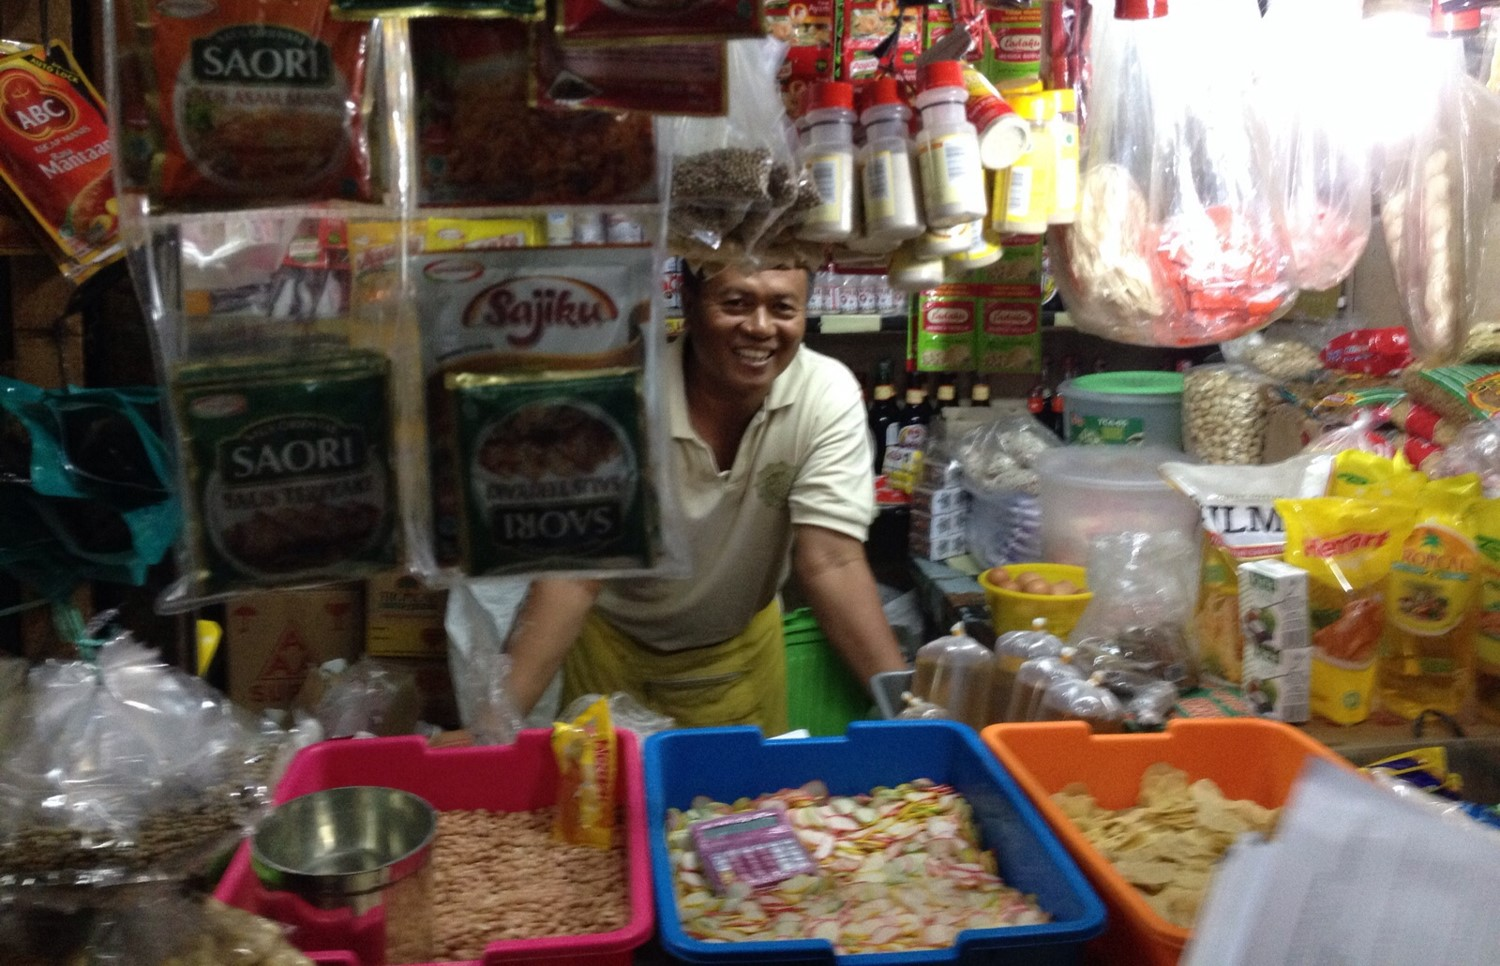
\includegraphics[width=4in]{pics/retailer1.jpg}
	%\caption{Best-practices handbook}
	\label{height}
\end{figure}
\end{frame}

\begin{frame}
\frametitle{Typical Business in the Sample}

\begin{figure}[htbp]
	\centering
		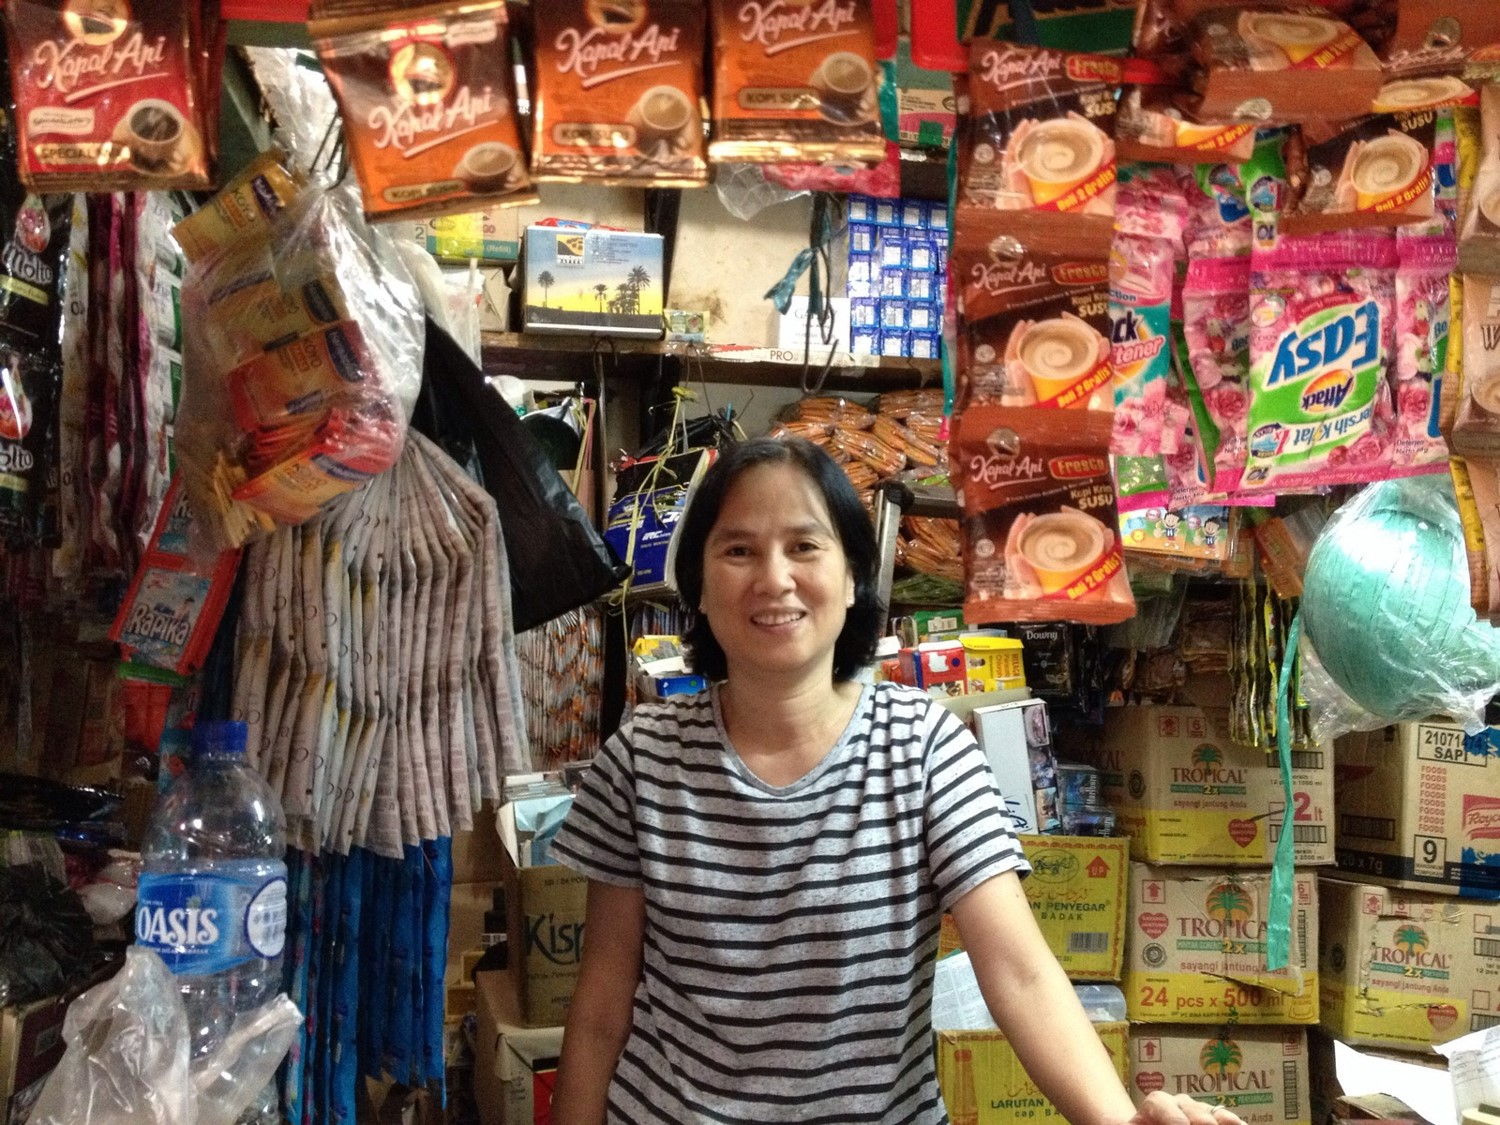
\includegraphics[width=4in]{pics/retailer2.jpg}
	%\caption{Best-practices handbook}
	\label{height}
\end{figure}
\end{frame}


\begin{frame}
\frametitle{Best-practices Handbook}

\begin{figure}[htbp]
	\centering
		
\includegraphics[width=4in]{pics/handbook.jpg}
	
	\label{height}
\end{figure}
\end{frame}


\begin{frame}
\frametitle{Handbook Content}
\begin{figure}[htbp]
	\centering
		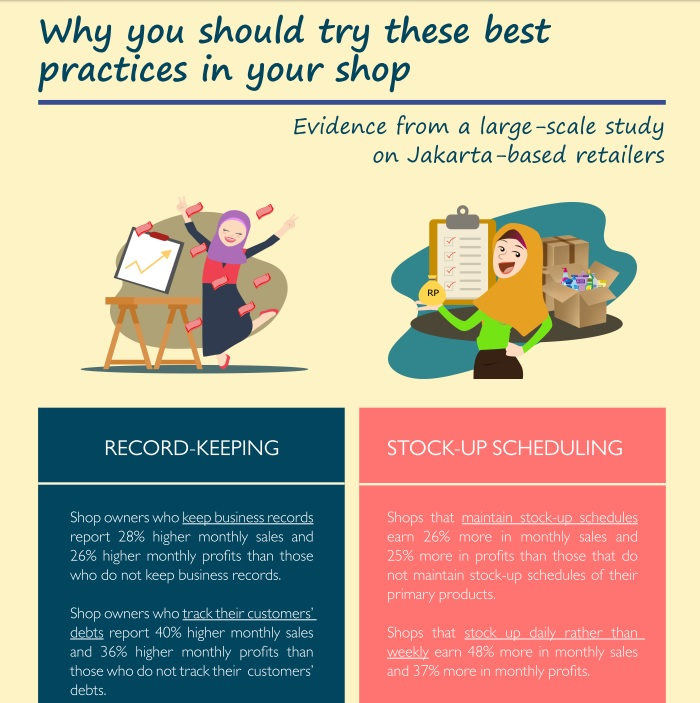
\includegraphics[width=2.6in]{pics/Handbook_return.jpg}
	
	\label{height}
\end{figure}
\end{frame}


%\begin{frame}
%\frametitle{Handbook Content}

%\begin{figure}[htbp]
%	\centering
%		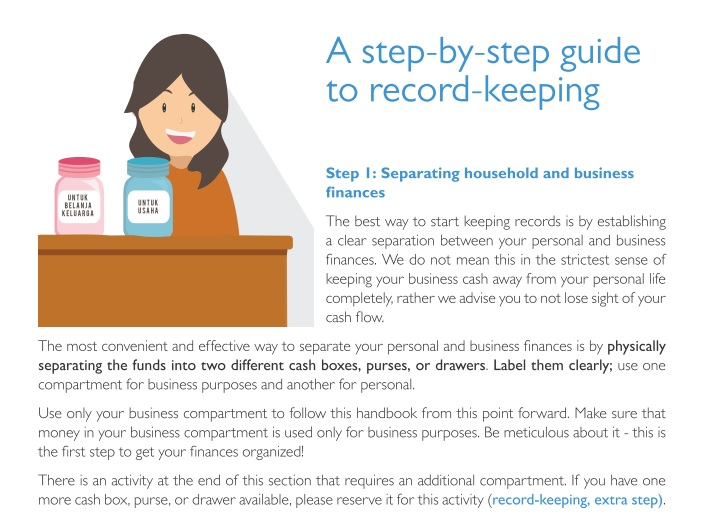
\includegraphics[width=2.6in]{pics/Handbook_stepbystep.jpg}
	
%	\label{height}
%\end{figure}
%\end{frame}

\begin{frame}
\frametitle{Movie with Successful Peers}
\begin{figure}[htbp]
	\centering
		\includegraphics[width=4.4in]{pics/movie.jpg}
   
	\label{height}
\end{figure}
\end{frame}


\begin{frame}
\frametitle{Implementation Assistance for Business Practices}
\begin{figure}[htbp]
	\centering
		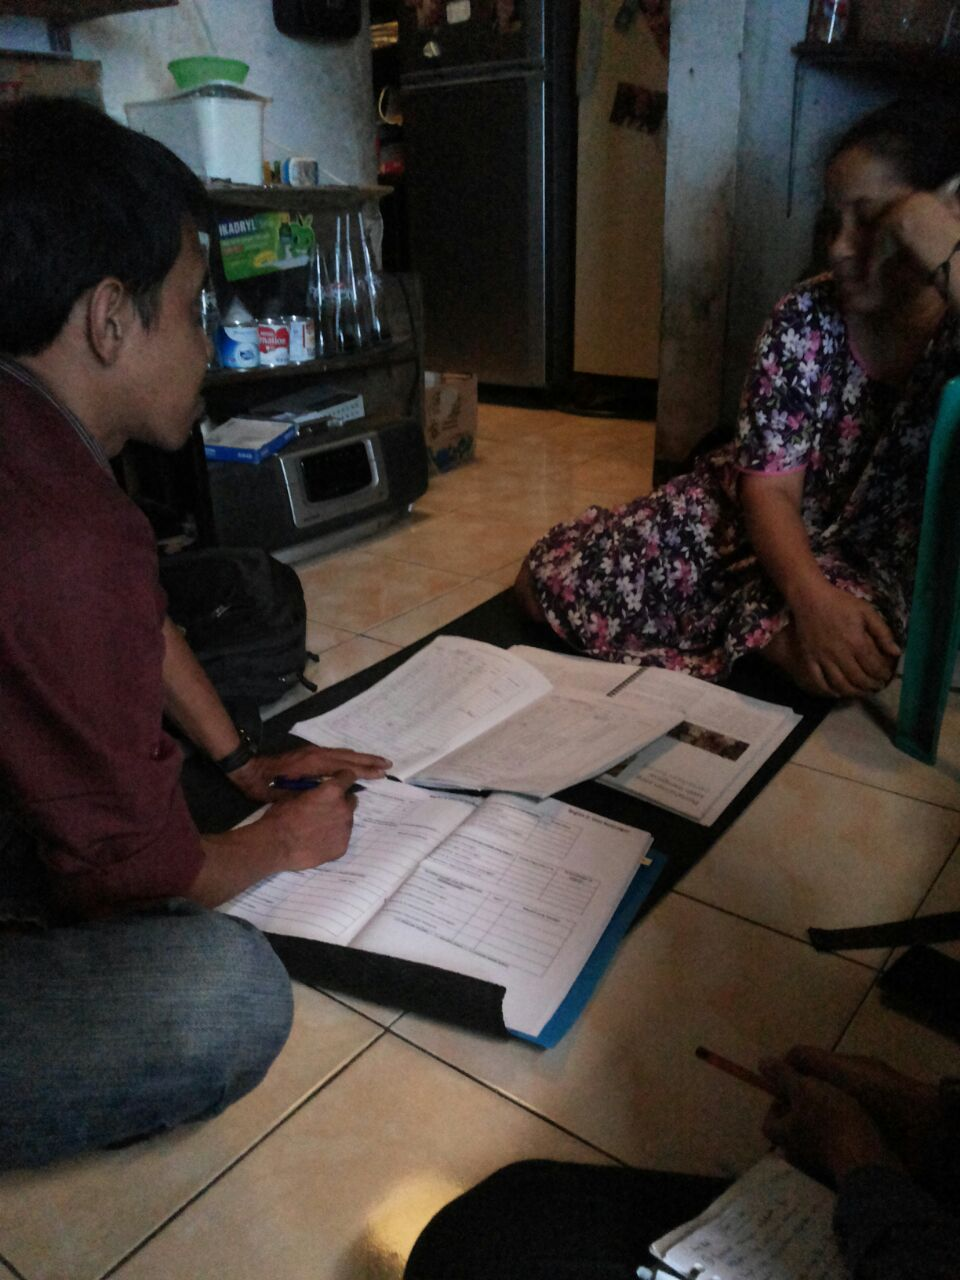
\includegraphics[width=2.0in]{pics/Assistance_expl.jpg}
	
	\label{height}
\end{figure}
\end{frame}


\subsection{Results}

\begin{frame}
\frametitle{Summary Statistics}

%\makebox[\linewidth][c]{
%\begin{tabular}{l cc ddd}


{\tiny{
	\begin{table}
		%\begin{adjustbox}{width=9.6cm}
		\centering	
		\tabcolsep=0.1cm
		\fontsize{5.2}{5.2}\selectfont

			\begin{tabular}{l*{10}{c}}
			\hline
			& (1)  &&(2) && (3)  &&(4) && (5) \\
			\hline


&\multicolumn{1}{c}{\textcolor{bdf}{Control}}
&&\multicolumn{1}{c}{\textcolor{bdf}{HB only}}	
&&\multicolumn{1}{c}{\textcolor{bdf}{HB \& MOV}	}
&&\multicolumn{1}{c}{\textcolor{bdf}{HB \& HELP}}	
&&\multicolumn{1}{c}{\textcolor{bdf}{HB \& MOV}}	\\


&\multicolumn{1}{c}{}
&&\multicolumn{1}{c}{}	
&&\multicolumn{1}{c}{}
&&\multicolumn{1}{c}{}	
&&\multicolumn{1}{c}{\textcolor{bdf}{\& HELP}}	\\


&\textit{N = 261}	
&&\textit{N = 260}	
&&\textit{N = 260}	
&&\textit{N = 260}	
&&\textit{N = 260}	\\
\hline \\

\textcolor{bdf}{Firm Owner Characteristics} \\
Gender (Male=1)											& 0.28	&& 0.3	&&0.29	&& 0.3	&& 0.28\\
Age														&45.22	&&45.27	&&45.28	&&45.16	&&45.38 \\
Education (Years)										&9.1	&&9.52	&&9.36	&&9.42	&&9.55 \\
%Digitspan												& 1.7	&& 1.67 && 	1.8 &&	1.67	&& 1.69 \\
														%&(1.12) 	&& 		&& 		&& 		&& 		&& \\
Risk Preference (0 - 10 ``Perfectly Risk-Seeking'')		&3.74	&&3.76	&&3.88	&&3.6	&&3.68 \\											
Time Preference	(0 - 10 ``Perfect Patience'')			&5.19	&&5.07	&&5.21	&&5.25	&&5.2 \\[0.5ex]
\\														
\textcolor{bdf}{Firm Characteristics} \\
Firm Age (Years)										&12.76		&&13.77		&&14.03		&&13.98		&&13.47 \\
Family Member Is Business Partner							&0.56		&&0.6		&&0.63		&&0.59		&&0.62 \\
Total Number of Workers									&2.03		&&2.05		&&1.9		&&1.99		&&2.04 \\
%Number of Full Time Paid Employees						&0.09		&&0.1		&&0.08		&&0.08		&&0.11		&&0.08 \\
														%&(0.3)		&&			&&			&&			&&			&& \\
Business Has Tax ID										&0.2		&&0.21		&&0.2		&&0.15		&&0.18 \\
Total Sales Last Month (USD PPP)						&4454.37 &&	4730.64	&& 4840.55	&& 4761.4	&& 5139 \\
												
Total Profits Last Month (USD PPP)						& 889.58	&& 961.1 &&	926.78	&& 825.25	&& 934.66 \\
Applied for Bus Loan in Last 12 Months
			    & 0.2	&& 0.17	&& 0.15	&& 0.22	&& 0.17 \\
													
Obtained Bus Loan in Last 12 Months
						& 0.18 &&	0.15	&& 0.14	&& 0.18	&& 0.14 \\[0.5ex]
\\
\textcolor{bdf}{Business Practices} \\
Management Practices Aggregate Score											& 0.37	&& 0.36	&& 0.37	&& 0.35	&& 0.37 \\
\hspace{3mm}Marketing Subscore												& 0.23	&& 0.23 &&	0.25	&& 0.23	&& 0.24 \\
\hspace{3mm}Stocking-up	Subscore											& 0.45	&& 0.47	&& 0.47	&& 0.47	&& 0.46 \\
\hspace{3mm}Record-keeping Subscore											& 0.33	&& 0.28	&& 0.3	&& 0.29 &&	0.3 \\
\hspace{3mm}Financial-planning Subscore									& 0.51	&& 0.47	&& 0.47	&& 0.43	&& 0.47 \\
%\hspace{3mm} Discussion Subscore                        & 0.57	&& 0.59	  && 0.61	&& 0.6	&& 0.64  \\
		\hline
			\end{tabular}
		%\end{adjustbox}			
		
		%\begin{adjustbox}{center}
			%\begin{tabular}{l*{12}{l}}
			%\multicolumn{13}{p{0.95\textwidth}}{\footnotesize \textit{Notes}: $^1$ Last month's sales and profits appear with both tails winsorized at 1%.}
			%\end{tabular}
		%\end{adjustbox}	
		
	\end{table}}}
%\end{tabular}

\vspace{-0.5em}

\begin{itemize_2pt}
\item[] \tiny Test of joint orthogonality from multinomial logit (p-value): \quad 0.857
\end{itemize_2pt}
\end{frame}


\begin{frame}
\frametitle{Movie: Take Up and Assessment}
{\scriptsize{\begin{table}[htbp]
%\fontsize{10}{11}\selectfont
  \centering
 	\fontsize{7}{7}\selectfont

    \tabcolsep=0.10cm
    %\begin{adjustbox}{width=11cm}
    \begin{tabular}{lcc}
    \hline
   	& (1)   					&(2)   						 \\
    \hline
  	& \textcolor{bdf}{HB \& MOV} 		& \textcolor{bdf}{HB \& MOV}		  \\
  	& 							& \textcolor{bdf}{\& HELP}			\\
   	& \textcolor{bdf}{(A)}   			& \textcolor{bdf}{(B)}   			 \\
 	&							&							\\
% 	&							&							&& \textit{F-test}\\
   	%	& Assigned 				& Assigned 					&&  \\
   	& \textit{N=260} 			& \textit{N=260} 			 \\
   \hline
   														&		&		 \\
    \textcolor{bdf}{Attendance} 								&       &         \\
  	% 													&		&		&& \\
    Business Owner or Partner Attended Film Screening 	& 0.52  & 0.49   \\
    %Baseline respondent attended film screening 		& 0.47  & 0.45  && 0.792 \\
   	%Respondent was reminded by phone 					& 0.05  & 0.07  && 0.355 \\
    %Respondent was reminded by visit to business 		& 0.35  & 0.33  && 0.782 \\
    %Distance to screening location (in decimal degrees)& 0.01  & 0.01  && 0.869 \\
	&       &       \\
    \textcolor{bdf}{Evaluation (1-4 Scale):}	&       &        \\
   	%									&       &       &&  \\
    Has Learned Something New	& 3.34  & 3.21  \\
    Feels Inspired 				& 3.31  & 3.30   \\
    Feels Hopeful 				& 3.60  & 3.42   \\
    Feels Bored 				& 0.83  & 0.97    \\
    \end{tabular}
   % \end{adjustbox}

\end{table}}}

\end{frame}


%%% Attendance and feedback to assistance + comparison between experimental groups
\begin{frame}

\frametitle{Assistance: Take Up and Assessment}
{\scriptsize{\begin{table}[htbp]
%\fontsize{10}{11}\selectfont
  \centering
  \fontsize{7}{7}\selectfont
    \tabcolsep=0.10cm
   % \begin{adjustbox}{width=11cm}
    \begin{tabular}{lcc}
    \hline
    & (1)   			& (2) 			\\
    \hline
   	& \textcolor{bdf}{HB \& HELP} 		& \textcolor{bdf}{HB \& MOV,}		 \\
  	& 							& \textcolor{bdf}{\& HELP}			 \\
   	& \textcolor{bdf}{(A)}   			& \textcolor{bdf}{(B)}   			\\
	&							&							 \\
% 	&							&							&& \textit{F-test}\\
   	%	&& Assigned 				& Assigned 					&&  \\
   	& \textit{N=260} 			& \textit{N=260} 		\\
    \hline
          																				&       &      \\
    \multicolumn{1}{l}{\textcolor{bdf}{Attendance}} 											&       &        \\
    %\multicolumn{1}{l}{\textit{1st session}} 											&       &       & &  \\
    \multicolumn{1}{l}{    Business Owner or Partner Attended 1st Session} 				& 0.77  & 0.78  \\
    %\multicolumn{1}{l}{    Baseline respondent attended 1st session} 					& 0.76  & 0.77  && 0.756 \\
    %\multicolumn{1}{l}{    Recipient plans to use at least one new practice} 			& 0.37  & 0.47  && 0.021** \\
    %\multicolumn{1}{l}{    Recipient plans neither handbook study nor implementation} 	& 0.12  & 0.11  && 0.784 \\
         														 						%&     	&       &&  \\
    %\multicolumn{1}{l}{\textit{2nd session}} 											&       &       &&  \\
    \multicolumn{1}{l}{    Business Owner or Partner Attended 2nd Session} 				& 0.68  & 0.68   \\
    %\multicolumn{1}{l}{    Baseline respondent attended 2nd session} 					& 0.67  & 0.67  && 1 \\
    %\multicolumn{1}{l}{    Recipient plans to use at least one new practice} 			& 0.39  & 0.47  && 0.063* \\
    %\multicolumn{1}{l}{    Recipient plans neither handbook study nor implementation} 	& 0.13  & 0.08  && 0.044** \\
          																				&       &        \\
    \multicolumn{1}{l}{\textcolor{bdf}{Evaluation (1-4 Scale)}} 								&       &         \\
    \multicolumn{1}{l}{Has Learned Something New} 										& 2.88  & 2.89   \\
    \multicolumn{1}{l}{Feels Inspired} 													& 2.76  & 2.83   \\
    \multicolumn{1}{l}{Feels Hopeful} 													& 2.88  & 2.97  \\
    \multicolumn{1}{l}{Feels Bored} 													& 0.59  & 0.43   \\
    \end{tabular}
   % \end{adjustbox}

\end{table}}}
\end{frame}


\begin{frame}
\frametitle{Impact on Business Practices}
\framesubtitle{Aggregate Scores}
{\tiny{\begin{table}[t]
%\centering
%\begin{adjustbox}{width=10cm}
\fontsize{5.5}{5.5}\selectfont
	\tabcolsep=0.10cm
	\begin{tabular}{l*{10}{c}}
		\hline
		\\
			&\textcolor{bdf}{Record}			&&\textcolor{bdf}{Planning}			&&\textcolor{bdf}{Stocking-up}	&&\textcolor{bdf}{Marketing} && \textcolor{bdf}{Joint} \\
&\textcolor{bdf}{Keeping}                       &&                        &&	                   &&	 && \textcolor{bdf}{Decision-making} \\
					&(1)					&&(2)						&&(3) 						&&(4) && (5)\\
			\cline{2-2}					\cline{4-4}					\cline{6-6}			\cline{8-8} \cline{10-10}  \\


Assigned Handbook 			&                    0.025   &&	          0.027   	 &&           -0.007   	 &&          -0.011   	  &&         0.011
      \\
         							&               (0.209)   	   &&      (0.273)   	&&         (0.694)   	     &&    (0.694)   	&&         (0.694)
    \\

         							
Assigned Handbook \& Movie 	&                     0.057*** 	 &&          0.043  	   &&       0.038  	    &&       0.040    &&        0.040        \\
          							&              (0.009)   &&	         (0.107)   	  &&       (0.117)   	  &&       (0.166)   	 &&        (0.217)         \\

         							
Assigned Handbook \& Assistance 	&              0.065*** 	  &&         0.034   	&&           0.011   	 &&           0.039 	       &&      0.037    \\
         							&           (0.004)   	  &&       (0.166)   &&	         (0.664)   && 	         (0.166)   	  &&       (0.239)    \\

         							
Assigned All Three          	&                0.054***	  &&         0.068***  	 &&          0.053**  	    &&       0.061**	   &&        0.059*          \\
									&             (0.009)    &&	         (0.009)   	&&         (0.020)   	  &&       (0.032)   &&	         (0.094)           \\

\hline         							
\\
R-squared									&               0.204   	 &&          0.192   	&&           0.187   	&&           0.150	 &&           0.120             \\
Sample Size 								&               2205   	  &&          2204   	   &&         2205   	 &&           2205   	    &&        2205      \\
Dependent Variable Mean of Control 		&                  0.196  	  &&         0.402   	 &&          0.471    &&	           0.250    	 &&          0.269          \\
Dependent Variable SD of Control 			&              0.252    	 &&          0.310   	  &&         0.270      	  &&         0.320    && 	           0.420        	\\
F-tests (p-value):							&			&&			&&			&&			\\
\hspace{5mm}Book = Book \& Mov				        &               0.069   	   &&           0.487   	  &&          0.014     	  &&          0.028    	 &&          0.300           \\
\hspace{5mm}Book = Book \& Assistance				        &               0.025  	  &&          0.754     	 &&           0.304   	 &&          0.030    	  &&          0.348                 \\
\hspace{5mm}Book = All Three				        &                  0.096    	  &&         0.073    	    &&      0.001   	  &&         0.002    &&	         0.082        \\
\hline
	\end{tabular}
%\end{adjustbox}
\end{table}}}
\begin{itemize}
\item[] \tiny Multiple hypothesis testing corrected p-values in parentheses
\end{itemize}

\begin{itemize}
\item \small ``All Three" improvement of 28 \% in record-keeping, 17 \% in planning, 11 \% in stocking, 24 \% in marketing and 22 \% in joint decision making.
\end{itemize}

\end{frame}


\begin{frame}

\frametitle{\centering{Business Profits}}
{\scriptsize{\begin{table}[t]
\centering
%\begin{adjustbox}{width=9cm}
\fontsize{5.7}{5.7}\selectfont
	\tabcolsep=0.10cm
	\begin{tabular}{l*{5}{c}}
\hline
&& (1) && (2) \\
\hline
			   &&\textcolor{bdf}{Profits}	        &&\textcolor{bdf}{Profits} \\
				&&\textcolor{bdf}{last month}  		&&\textcolor{bdf}{last month} \\
			&&(win 5\%)			&&(IHS) \\
				&&(1)				&&(2)	\\
&& \\
					\hline
&&\\
		

Assigned Handbook 					&&-91.307   	&& -0.067   		\\
       								 	&&         (78.400)  	&&          (0.088)  	\\

         							
Assigned Handbook \& Movie				&&110.378   	  	&& 0.055   		\\
       									&&         (86.841)  	&&          (0.092)  	\\

         							
Assigned Handbook \& Assistance 	&&         310.455***	&&           0.261***		\\
       								 	&&         (89.488) 	&&          (0.096)  	\\
         							
Assigned All Three          		&&         191.088**  	&&           0.199** 		\\
       								 	&&         (84.662)  	&&          (0.094)  	\\

   	\\
\hline         							
\\
R-squared											  	&& 0.179  	&& 0.211  	\\
Sample Size 											&&2172	&& 2172 	\\
Dependent Variable Mean in Control Group			 	&&          894.544   	&&           6.817 	\\
Dependent Variable SD in Control Group				 	&&         1127.783   	 &&          1.348  	\\
F-tests (p-value):											&&			&&			\\
\hspace{5mm}Book = Book \& Mov				        	&&    0.020   	&&            0.167 	\\
\hspace{5mm}Book = Book \& Assistance				  			&&0.000   	&&0.000  	\\
\hspace{5mm}Book = All Three			   			  	&&0.001   	&&0.003  	\\
\hline
	\end{tabular}
%\end{adjustbox}

\end{table}}}

\vspace{-0.5em}

\begin{itemize_2pt}
\item Intention to treat (ITT): Profits increase by 35\% (about 0.28 sd.)
\end{itemize_2pt}
\end{frame}




\begin{frame}
\frametitle{Business Sales}
{\scriptsize{\begin{table}[t]
\centering
%\begin{adjustbox}{width=9cm}
\fontsize{5.7}{5.7}\selectfont
	\tabcolsep=0.10cm
	\begin{tabular}{l*{5}{c}}
\hline
&& (1) && (2) \\
\hline
                &&\textcolor{bdf}{ITT}	        &&\textcolor{bdf}{TOT} \\
			   &&\textcolor{bdf}{Sales}	        &&\textcolor{bdf}{Sales} \\
				&&\textcolor{bdf}{last month}  		&&\textcolor{bdf}{last month} \\
			&&(win 5\%)			&&(win 5\%) \\
				&&(1)				&&(2)	\\
&& \\
					\hline
&&\\
		

Assigned Handbook 					&&-396.976   	&&               -417.198		\\
       								 	&&        (314.252)   	&&          (-397.174)	\\

         							
Assigned Handbook \& Movie				&&335.489   	  	&& 601.221    		\\
       									&&       (337.881)  	&&            (606.634)	\\

         							
Assigned Handbook \& Assistance 	&&                   836.755**	&&                     1031.692** 	\\
       								 	&&        (372.924) 	&&            (457.015) 	\\
         							
Assigned All Three         		&&         807.462**  	&&                         1558.326**		\\
       								 	&&        (358.384)  	&&          (696.317)   	\\

   	\\
\hline         							
\\
R-squared											  	&& 0.492  	&&  0.483	\\
Sample Size 											&& 2197	&& 2197 	\\
Dependent Variable Mean in Control Group			 	&&         4998.923   &&	          4998.923 	\\
Dependent Variable SD in Control Group				 	&&         5623.257   	&&           5623.257	\\
F-tests (p-value):											&&			&&			\\
\hspace{5mm}Book = Book \& Mov				        	&&            0.020 	&&           0.047 	\\
\hspace{5mm}Book = Book \& Assistance				  			&&0.000   	&& 0.000 	\\
\hspace{5mm}Book = All Three			   			  	&&0.000   	&&0.001  	\\
\hline
	\end{tabular}
%\end{adjustbox}

\end{table}}}

\vspace{-0.5em}

\begin{itemize_2pt}
\item Intention to treat (ITT): Sales increase by 16\% (about 0.15 sd.)
\end{itemize_2pt}
\end{frame}


\begin{frame}
\frametitle{Other Outcomes}

\textcolor{bdf}{No significant impacts} on:
    \begin{itemize_2pt}
    \vspace{0.1in}
    \item Business expenses
    \vspace{0.1in} 		
    \item Business size
      \vspace{0.1in}
    \item Number of employees
      \vspace{0.1in}
    \item Number of customers
       \vspace{0.1in}
     \item Business credit
    \end{itemize_2pt}

\end{frame}

\subsection{Discussion}
\begin{frame}
\frametitle{Efficiency Gains?}
Impact on business practices $\rightarrow$ \textcolor{bdf}{efficiency practices}:
\vspace{0.1in}
\begin{itemize_2pt}
	\item Adjust stocks based on product profitability
	\item Negotiate lower prices with suppliers
	\item Consult with former customers
	\item Offer discounts
	\item Make joint decisions
	\item Review performance to identify ways to improve
	\item Make anticipated budget for upcoming costs

	\pause
	
	\item[] $\rightarrow$ \textcolor{bdf}{Non-record-keeping practices}
	\item[] $\rightarrow$ Causal mediation analysis: \textcolor{bdf}{Stocking up and marketing practices} drive performance impact
	\item[] $\rightarrow$ Variance in profits among treated firms does not converge
	\item[] $\rightarrow$ \textcolor{bdf}{Efficiency gains}
\end{itemize_2pt}
\end{frame}

\begin{frame}
\frametitle{Business Knowledge or Aspirations?}
Impact on practice adoption and business performance may work through ..
\begin{itemize_2pt}
	\item .. acquisition of \textcolor{bdf}{business knowledge} and/or
	\item .. strengthening of \textcolor{bdf}{growth aspirations}
\end{itemize_2pt}

\pause
\vspace{1.0em}

We directly measure \textcolor{bdf}{business aspirations} .. 
\begin{itemize_2pt}
	\item .. at baseline, midline, and endline
	\item .. for short (one year) and long ("ideal business") time horizons
	\item .. for various dimensions of potential business expansion
    \begin{itemize_2pt}
   		\item Sales on a normal day
    	\item Physical size
   		\item Customers on a normal day
    	\item Employees
    \end{itemize_2pt}
\item[] $\rightarrow$ \textcolor{bdf}{No impact on aspirations}
\item[] $\rightarrow$ Performance likely driven by increase in \textcolor{bdf}{business knowledge}
\end{itemize_2pt}

\end{frame}

\begin{frame}
\frametitle{Business Stealing?}
Do treated businesses improve performance at the expense of the control?
\vspace{0.1in}
\begin{itemize_2pt}
\item Sales and profits of \textcolor{bdf}{control businesses do not decrease} from baseline to endline (roughly equal)
\item Sales and profits of control businesses \textcolor{bdf}{closer to treated shops do not decrease by more} than those further away
\item[] $\rightarrow$ \textcolor{bdf}{No evidence for business stealing}
\end{itemize_2pt}
\end{frame}

\begin{frame}
\frametitle{Cost-Effectiveness}

\textcolor{bdf}{Small costs (per firm)}:
\begin{itemize_2pt}
\item Cost Handbook alone: USD 100
\item Cost Handbook \& Movie: USD 125
\item Cost Handbook \& Assistance: USD 125
\item Cost Handbook \& Movie \& Assistance: USD 150
\end{itemize_2pt}
\vspace{0.5em}

\textcolor{bdf}{Substantial Benefits}
\begin{itemize_2pt}
\item Up to USD 330 per month in profits
\item Adoption of top practices by retailers
\end{itemize_2pt}

\vspace{0.5em}
Research design likely \textcolor{bdf}{scalable and portable}

\end{frame}

\subsection{Conclusion}
\begin{frame}
\frametitle{Takeaways}
\begin{itemize_2pt}
    \item \textcolor{bdf}{Curating local knowledge has value for business growth} 
    \item Information alone does not have impact, only combined with \textcolor{bdf}{behavioral interventions}
    \item Mechanism likely \textcolor{bdf}{knowledge-based}, not aspirations-based
	\item Behavioral interventions are \textcolor{bdf}{inexpensive and scalable}
	\item[] $\rightarrow$  Attractive for policy
    
\end{itemize_2pt}
\end{frame}


\begin{frame}
\frametitle{Questions}

\textcolor{bdf}{Any questions?}
\begin{itemize_2pt}
    \item[] .. happy to stay on for a little while!
\end{itemize_2pt}
\end{frame}





%\addtocontents{toc}{\protect\setcounter{tocdepth}{0}}

\appendix
\begin{frame}[allowframebreaks] %label=references, 
\frametitle{References}
\bibliographystyle{chicago}
\bibliography{businessTraining}
\end{frame}


\section*{\textbf{Appendix}}

\setbeamertemplate{sidebar right}[sidebar theme]

%\begin{frame}{Appendix Overview}
%\tableofcontents[currentsection,hideothersubsections]
%\end{frame}


\begin{frame}[label=McK2020_sales]
\frametitle{Evidence of Impact}

	\begin{figure}[htbp]
		\centering
		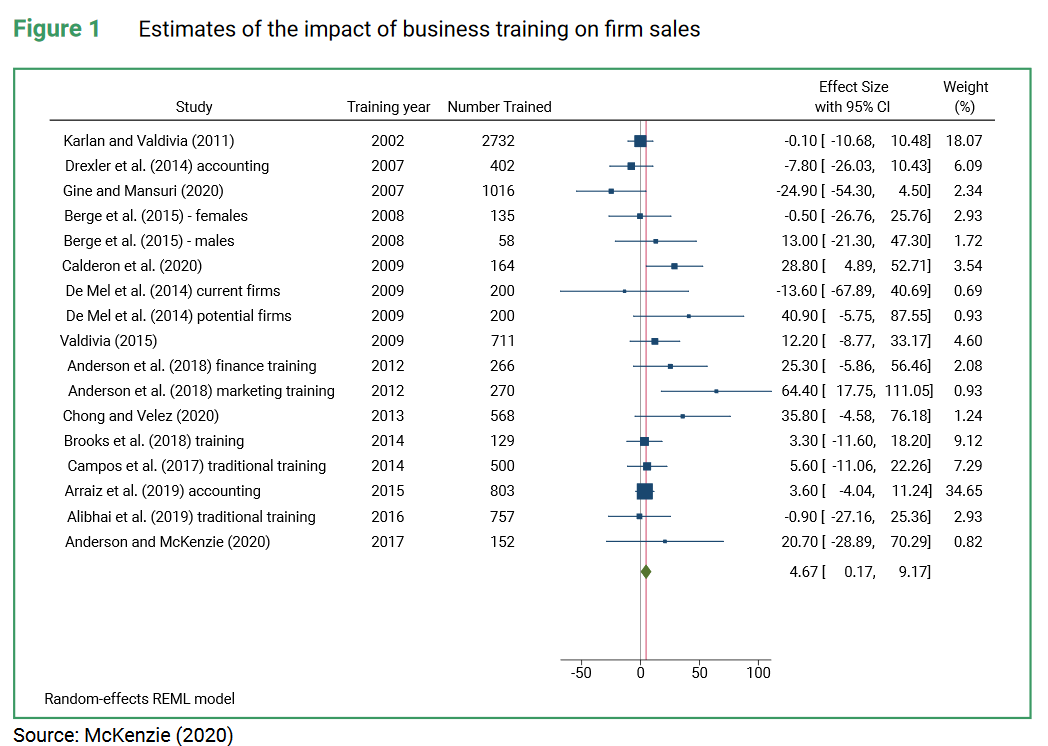
\includegraphics[width=23.2em]{pics/McK2020_sales.png}
		\label{McKenzie(2020): Sales}
	\end{figure}	
	
	\vspace{-1em}	
	
	\begin{itemize_2pt}
		\item Small positive impact on sales (back to \hyperlink{McK2020_profits}{\beamergotobutton{profits}})
	\end{itemize_2pt}
	
\end{frame}


\end{document}
